\documentclass[12pt]{report}
\usepackage[left=3cm, right=3cm, top=3cm]{geometry}
\usepackage[utf8]{inputenc}
\usepackage{graphicx}
\graphicspath{ {images/} }
\usepackage{amsmath}
\renewcommand{\vec}{\mathbf}
\usepackage{todonotes}
\usepackage{wrapfig}
\usepackage[font=scriptsize]{caption}
\usepackage{mwe}
\usepackage{multicol}
\usepackage{subfig}
\usepackage{float}
\usepackage{amsmath,tabularx}
\usepackage{booktabs}
\usepackage[normalem]{ulem}
\usepackage[T1]{fontenc}
\renewcommand{\vec}{\mathbf}
\usepackage[utf8]{inputenc}
\useunder{\uline}{\ul}{}
\usepackage[colorlinks=true, citecolor=blue, linkcolor=black, urlcolor=black]{hyperref}




\begin{document}

\pagenumbering{gobble}

\begin{center}
\textbf{\Huge POLITECNICO DI TORINO}

\begin{figure}[H]
  \centering
  
\includegraphics[width=2.5in]{poli.png}
\end{figure}

\end{center}
\begin{center}
\vspace{0.05in}
\Large{\textbf{ICT For Smart Societies}\\
\vspace{0.08in}
\Large ICT for Health (Lab 1)}\\
\large Prof. Monica Visintin
\end{center}
\begin{center}
\vspace{0.08in}
\end{center}

\begin{center}
\textbf{\Huge REGRESSION\\ on\\ PARKINSON DATA\\}
\end{center}


\begin{center}
\vspace{1in}
\textbf{\Large GENNARO RENDE}\\
\textbf{S218951}\\
\end{center}


\pagebreak

\pagenumbering{gobble}

\tableofcontents


\chapter{Introduction}
\pagenumbering{arabic}
\section{Parkinson's Disease}
Parkinson's disease affects patients, not enabling them to control their muscles (difficulties in starting a movement) and also to control their voice because of the rigidity of the muscles' vocal cords. Patients who suffer from this disease, are given certain amounts of Levodopa, which acts by transforming itself, in the organism, into dopamine: a neurotransmitter responsible, among other things,  of the movement's control.
\section{The medical issue}
"This illness is under the check of neurologists who judge the state of health of their patients by asking them to perform different movements. This type of control has the purpose of optimizing the therapy, which consists in taking a precise amount of Levodopa. It is difficult for neurologists to regulate the treatment because of the continuous progression of the illness. All the movements made by the patient, during the check, are numerically evaluated and summed: this is the final grade, which is called total UPDRS (Unified Parkinson's Disease Rating Scale).
To improve the research, for each patient, It would be useful to find an automatic way to give them an objective score, which can be measured several times during the day and help the neurologist to optimize, in the best way possible, the treatment." \cite{MV1}

\section{The Data}
"This dataset is composed of a range of biomedical voice measurements from 42 people with early-stage Parkinson's disease recruited to a six-month trial of a telemonitoring device for remote symptom progression monitoring. The recordings were automatically captured in the patient's homes.
Columns in the table contain subject number, subject age, subject gender, time interval form baseline recruitment date, \texttt{UPDRS}\textsubscript{\textbf{motor}}, \texttt{UPDRS}\textsubscript{\textbf{total}} and 16 biomedical voice measures. Each row corresponds to one of 5.875 voice recording from these individuals. The main aim of the data is to predict the motor and the \texttt{UPDRS}\textsubscript{\textbf{total}} scores from the 16 voice measures." \cite{site}
\subsection{Managing the data}
"We use the first 50\% of the rows of data as \textbf{training points}, the subquent 25\% as \textbf{validation points and the remaining 25\% of the rows as \textbf{testing points}}."\cite{MV1}
\subsection{Standardization of the data}
Standardization is often used to avoid biased results because it centers the data around zero and divides them by their standard deviation.This procedure makes comparable all the features. A not standardized matrix requires the addition of a column of ones, giving the data a dimension of \textit{N} $\times$ \textit{F+1}. In the case the real model remains non standardized, it has an offset and we have a matrix of \textit{F} dimensions; this case, won't be able to predict new data. Standardization eliminates offsets such that we can solve the Regression problem in \textit{F} dimensions.
\section{Regression Analysis}
"In statistical modeling, regression analysis is a set of statistical processes for estimating the relationships among variables. It provides modeling and analysis of several variables, when the focus is on the relationship between a dependent variable and one or more independent variables (or 'predictors'). Regression analysis helps one understand how the typical value of the dependent variable (or 'criterion variable') changes when any one of the independent variables is varied, while the other independent variables are held fixed."\cite{WikiRegression} The modus operandi we will follow is regressing the feature \texttt{UPDRS}\textsubscript{\textbf{total}} from the other features with different algorithms. The matrix $\textbf{X}$ will contain all the features except \texttt{UPDRS}\textsubscript{\textbf{total}}, the column vector $\textbf{y}$ will instead filled only with the feature that $\textbf{X}$ is missing. The correlation between these data structures will allow us to find the vector $\hat { \mathbf { w } }$ which data represent how much each feature of $\textbf{x}$ is correlated to $\textbf{y}$.
Eventually, a new vector $\hat { \mathbf { y } }$ containing the regressed feature \texttt{UPDRS}\textsubscript{\textbf{total}} can be obtained by:
\begin{equation}
\hat { \mathbf { y } } = \mathbf { X } \hat { \mathbf { w } }
\end{equation}

Some of the algorithms require a lot of iterations in order to find $\hat { \mathbf { w } }$ , for this reason it is useful to impose a stopping condition in order to stop the algorithm when the improvement of the solution becomes too small:

\begin{equation}
\left\| \hat { \mathbf { w } } _ { i + 1 } - \hat { \mathbf { w } } _ { i } \right\| < \epsilon
\end{equation}



\chapter{Algorithms}
To have constant results we used the "seed" function in Python (in this case with number \textbf{2}), $\mathbf{\epsilon=10^{-4}}$ and $ \mathbf{\gamma=10^{-5}}$
\section{Linear Least Square}
In our study we did $n$ measurements:
$y ( n ) = \mathbf { x } ^ { T } \mathbf { w } + \boldsymbol{ \nu}$ ($\boldsymbol{ \nu}$ is a measurement error) ending up with matrices settled in this way:
\begin{tiny}
\begin{equation}
\small
\vec{X}=
\begin{bmatrix}
x_1(1) & x_2(1) & x_2(1) & \dots & x_F(1) \\
x_1(2) & x_2(2) & x_2(2) & \dots & x_F(2)\\
x_1(3) & x_2(3) & x_2(3) & \dots & x_F(3) \\
\vdots & \vdots & \vdots & \ddots & \vdots \\
x_1(N) & x_2(N) & x_2(N) & \dots & x_F(N)
\end{bmatrix}
=
\begin{bmatrix}
\vec{x}^T(1) \\
\vec{x}^T(2) \\
\vec{x}^T(3) \\
\vdots \\
\vec{x}^T(N) \\
\end{bmatrix}
;\quad
\vec{y}=
\begin{bmatrix}
y(1) \\
y(2) \\
y(3) \\
\vdots \\
y(N) \\
\end{bmatrix}
\end{equation}
\end{tiny}


\begin{equation}
\text{we have: }
\mathbf { y } = \mathbf { X } \mathbf { w } + \boldsymbol { \nu }
\end{equation}
\textbf{y} are our measurements, while $\textbf{X}$ is a data-matrix of $\textbf{N}$ rows (the number of patients) and \textit{F} columns (their features). Our intent is to find the optimum \textbf{w} (the solution) to minimize the square error: $f ( \mathbf { w } ) = \| \mathbf { y } - \mathbf { X w } \| ^ { 2 }$.
Calculating the expression $\nabla f ( \mathbf { w } ) =0 $ we then find the optimum ${ \mathbf { w } }$ as: $\hat { \mathbf { w } } = \left( \mathbf { X } ^ { T } \mathbf { X } \right) ^ { - 1 } \mathbf { X } ^ { T } \mathbf { y }$
\subsection{Results}
In Figure\textbf{\subfigurename~\ref{fig:lls_a}} and\textbf{\subfigurename~\ref{fig:lls_b} }we see how the train data behave: the scattering plot well surrounds the diagonal (which represents the values that are supposed to show up) and the histogram has a Gaussian distribution with $\mu = 0$, meaning that our results mostly have an error around $0$. In Figure\textbf{\subfigurename~\ref{fig:lls_c}} and\textbf{\subfigurename~\ref{fig:lls_d}} we see how the test data performed and, seeing the good results of our trained data, we receive a fine equal performance.
Finally we check the Figure\textbf{\subfigurename~\ref{fig:lls_e}} that shows of the optimum result depends especially on the values of \texttt{Shimmer}\textsubscript{\textbf{APQ3}}, \texttt{Shimmer}\textsubscript{\textbf{DDA}}, and \texttt{UPDRS}\textsubscript{\textbf{motor}}.
\pagebreak

\begin{center}
\subsubsection{Results with the "Linear Least Square" Algorithm}
\end{center}

\begin{figure}[H]
\centering
\begin{center}
\subfloat[][\emph{$\hat { \mathbf { y } } _ { \mathrm { train } } \textit{{\scriptsize VS} }  \mathbf {y } _ { \mathrm { train } }$}\label{fig:lls_a}]
{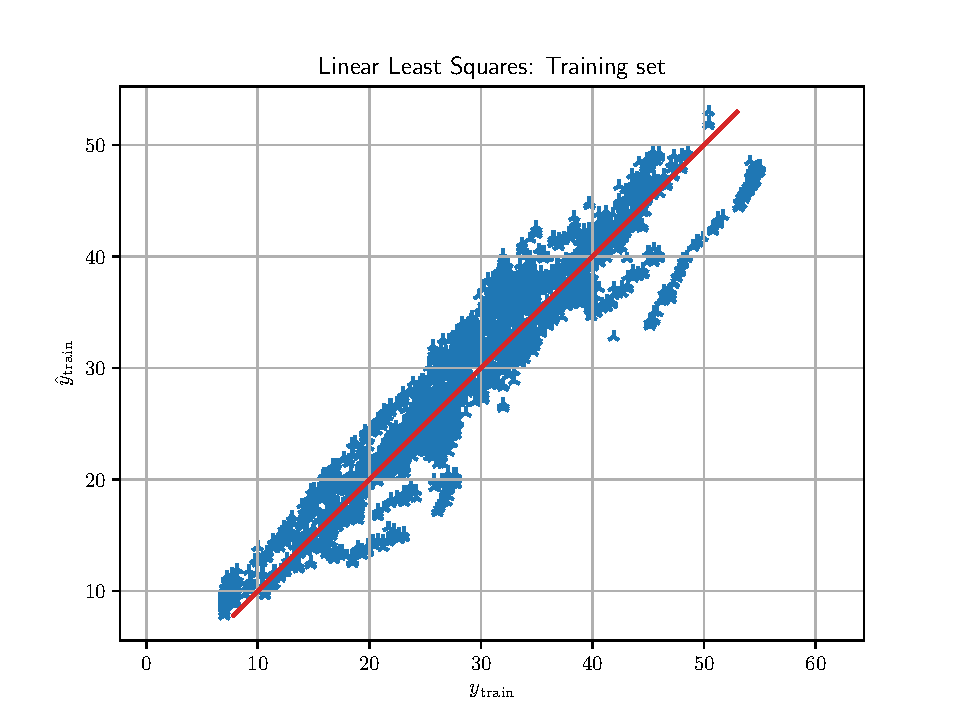
\includegraphics[width=.5\textwidth]{s_train_Linear_Least_Squares.pdf}}
\subfloat[][\emph{$\hat { \mathbf { y } } _ { \mathrm { train } } \textit{{\scriptsize -} }  \mathbf {y } _ { \mathrm { train } }$}\label{fig:lls_b}]
{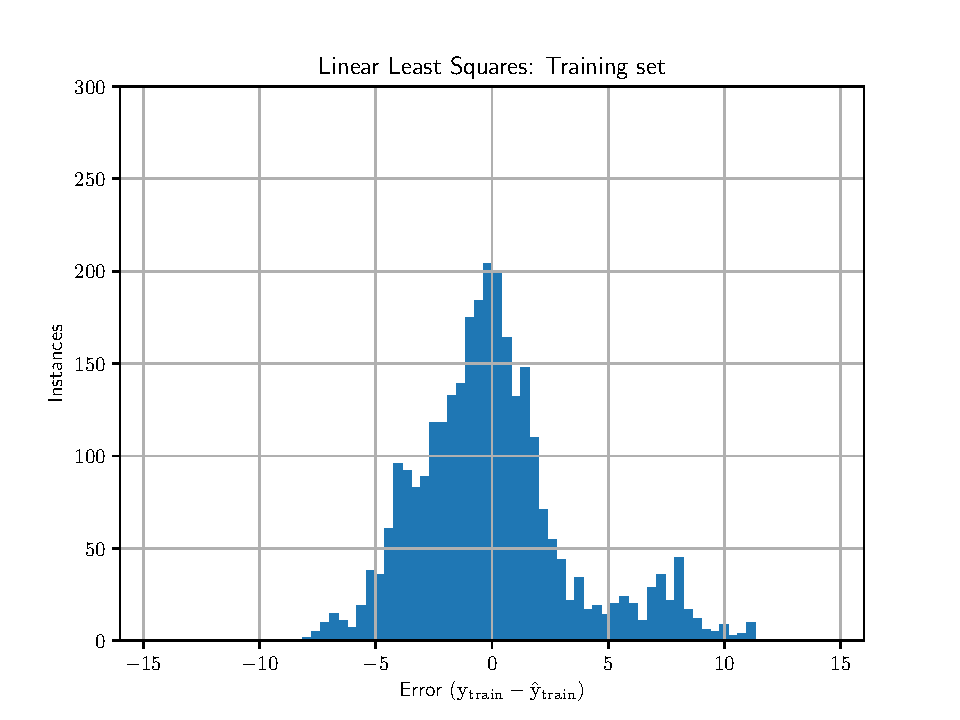
\includegraphics[width=.5\textwidth]{h_train_Linear_Least_Squares.pdf}}\\
\subfloat[][\emph{$\hat { \mathbf { y } } _ { \mathrm { test } } \textit{{\scriptsize VS} }  \mathbf {y } _ { \mathrm { test } }$}\label{fig:lls_c}]
{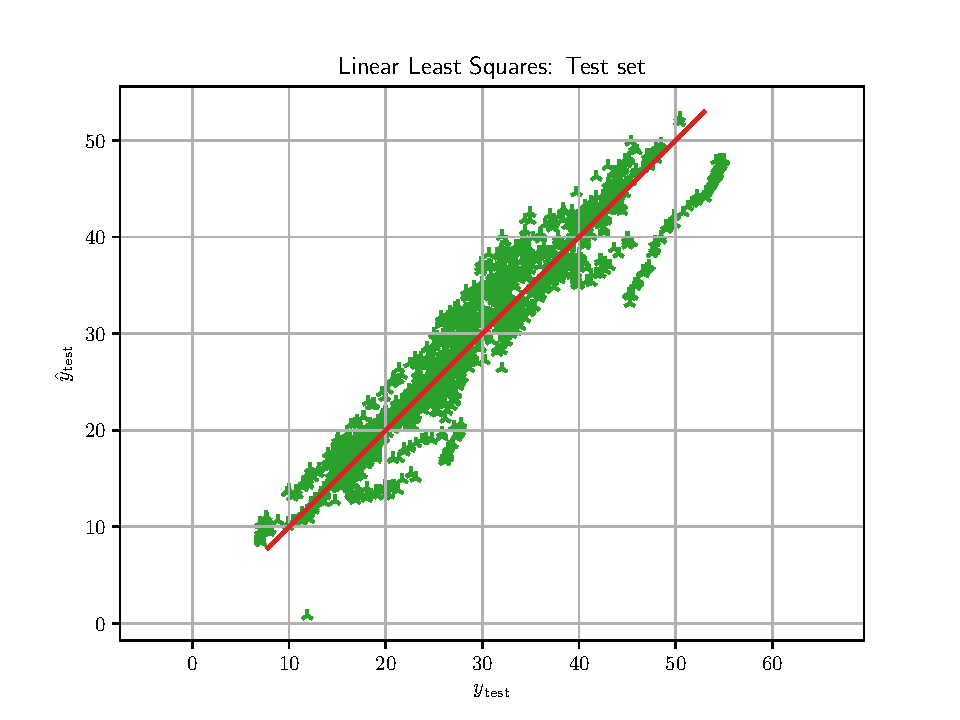
\includegraphics[width=.5\textwidth]{s_test_Linear_Least_Squares.pdf}}
\subfloat[][\emph{$\hat { \mathbf { y } } _ { \mathrm { test } } \textit{{\scriptsize -} }  \mathbf {y } _ { \mathrm { test } }$}\label{fig:lls_d}]
{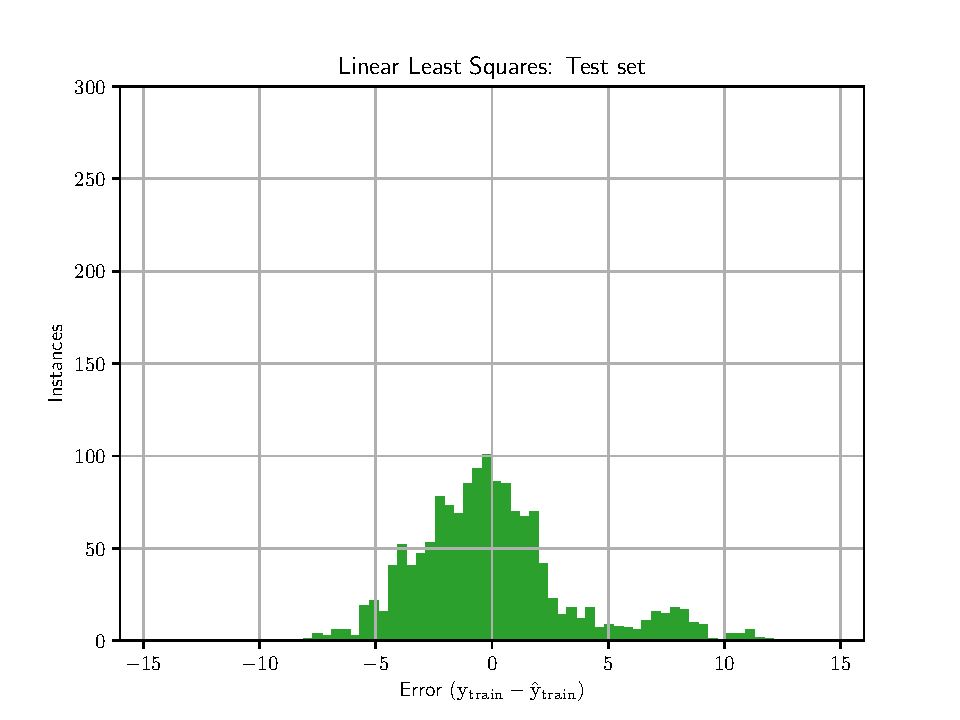
\includegraphics[width=.5\textwidth]{h_test_Linear_Least_Squares.pdf}}\\
\subfloat[][\emph{Optimum $\textbf{w}$ for every feature}\label{fig:lls_e}]
{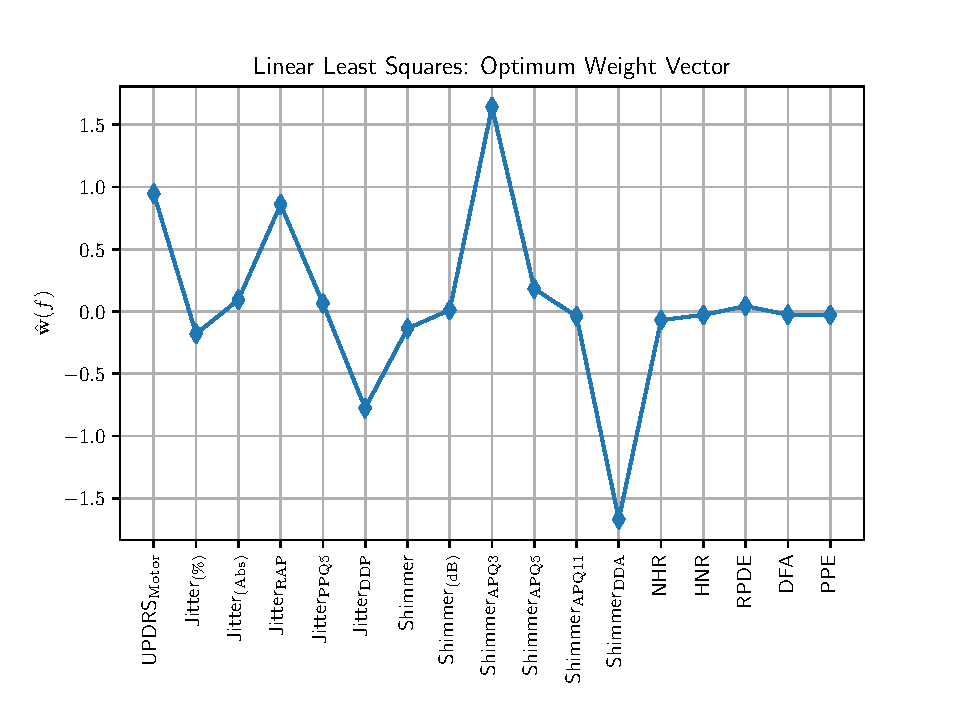
\includegraphics[width=.5\textwidth]{w_Linear_Least_Squares.pdf}}
\caption{Linear Least Square}
\label{fig:lls}
\end{center}
\end{figure}






\section{Gradient Descent}\label{gr}
"Gradient descent is a first-order iterative optimization algorithm for finding the minimum of a function. To find a local minimum of a function using gradient descent,one takes steps proportional
 to the negative of the gradient (or approximate gradient) of the function at the current point."\cite{GD}
 This minimization algorithm relies to the fact that the
\begin{wrapfigure}{r}{0.4\textwidth}
  \vspace{-20pt}
  \begin{center}
    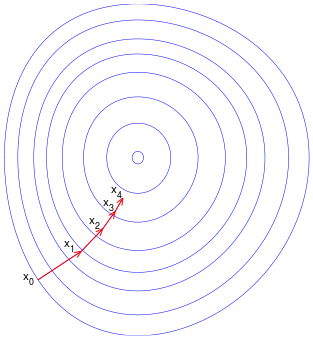
\includegraphics[width=0.32\textwidth]{GD.png}
    \caption{Gradient Descent \cite{GD}}
    \label{fig:graddesc}
  \end{center}
  \vspace{-10pt}
  \vspace{-10pt}
\end{wrapfigure}
maximum descent direction in a point of a function is the opposite of the direction of the gradient in that point.
After having evaluated the gradient as
 \begin{equation}
  \nabla f ( \mathbf { w } ) = 2 \mathbf { X } ^ { \top } ( \mathbf { X w } - \mathbf { y } )
\end{equation}
we chose the learning coefficient $\gamma$ and iterate for a discrete number of iterations:
\begin{equation}\label{2.4}
\mathbf { w } _ { i + 1 } = \mathbf { w } _ { i } - \gamma \nabla f \left( \mathbf { w } _ { i } \right)
\end{equation}
In the end the vector \textbf{w} converges to an optimum solution to reach the point of minimum of the function as in [\figurename~\ref{fig:graddesc}]

\subsection{Results}
Also in this case the output of $\hat { \mathbf { y } }$ is well performed, as we can see in [\textbf{\ref{fig:gradd_a}}] and the error shown in [\textbf{\ref{fig:gradd_b}}] confirms how little it affects the results since the $\mu = 0$.
On the other hand we see a different result for the output of the $\hat { \mathbf { w } }$: the feature that has a significant correlation with \texttt{UPDRS}\textsubscript{\textbf{total}} is \texttt{UPDRS}\textsubscript{\textbf{motor}} while the others have a little impact (exception made for \texttt{Shimmer} and \texttt{Shimmer}\textsubscript{\textbf{APQ5}}).
The figure [\textbf{\ref{fig:gradd_f}}] shows the trend of the Mean Square Error VS the number of iterations made to improve the result of $\hat { \mathbf { w } }$: after almost 500 iterations, the training set, the test set and the validation set have the same trend and values and no overfitting is seen since the two functions almost overlap.


\begin{center}
\subsubsection{Results with the "Gradient Descent" Algorithm}
\end{center}
\begin{figure}[H]
\centering
\subfloat[][\emph{$\hat { \mathbf { y } } _ { \mathrm { train } } \textit{{\scriptsize VS} }  \mathbf {y } _ { \mathrm { train } }$}\label{fig:gradd_a}]
{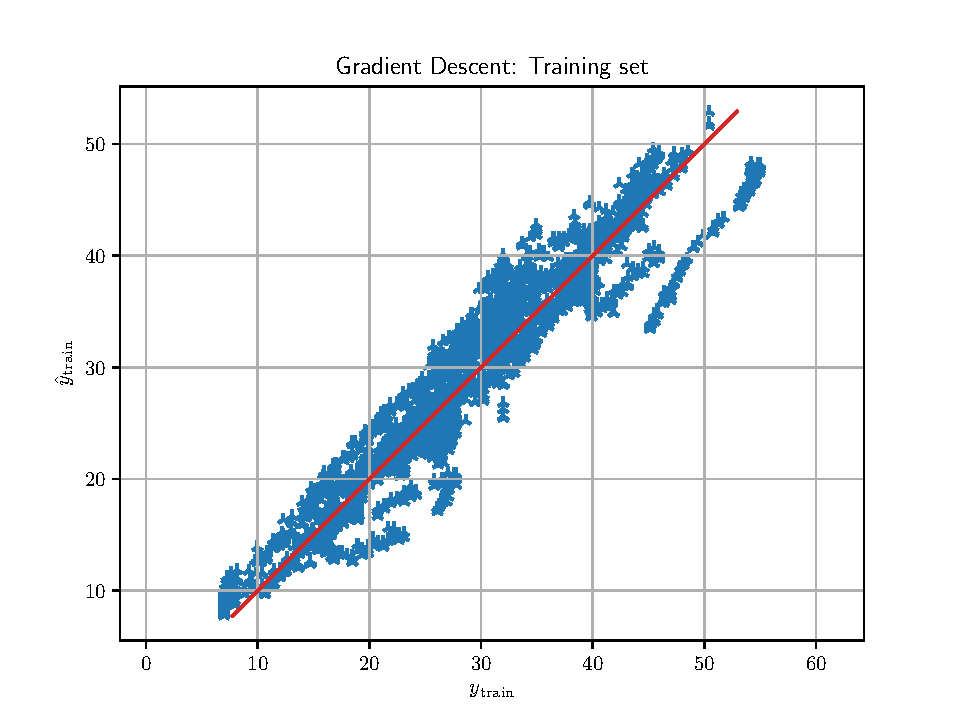
\includegraphics[width=.5\textwidth]{s_train_Gradient_Descent.pdf}}
\subfloat[][\emph{$\hat { \mathbf { y } } _ { \mathrm { train } } \textit{{\scriptsize -} }  \mathbf {y } _ { \mathrm { train } }$}\label{fig:gradd_b}]
{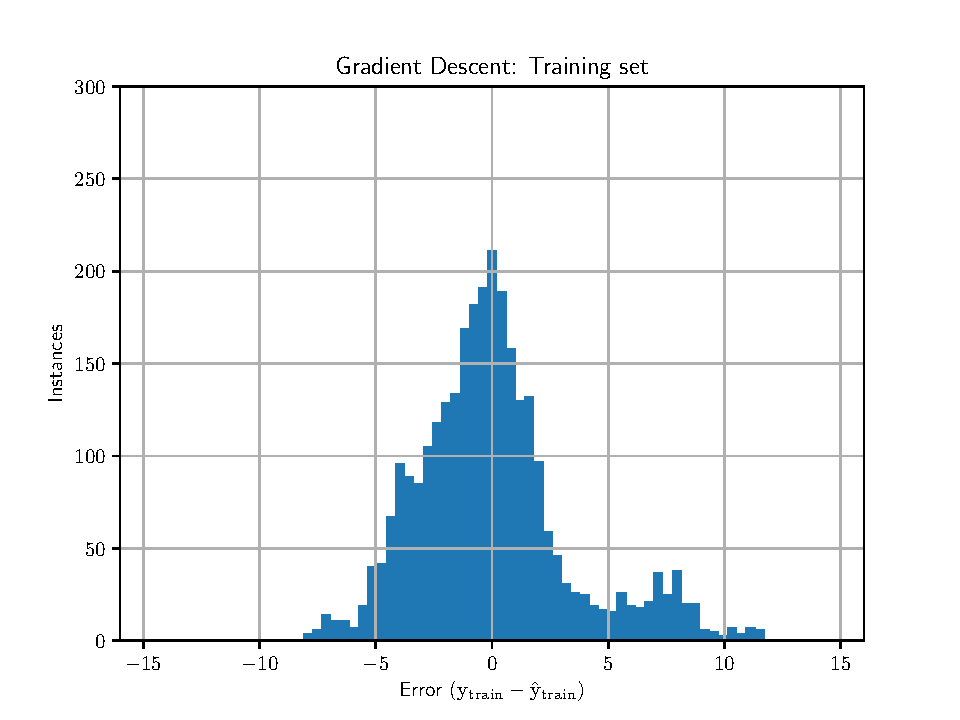
\includegraphics[width=.5\textwidth]{h_train_Gradient_Descent.pdf}}\\
\subfloat[][\emph{$\hat { \mathbf { y } } _ { \mathrm { test } } \textit{{\scriptsize VS} }  \mathbf {y } _ { \mathrm { test } }$}\label{fig:gradd_c}]
{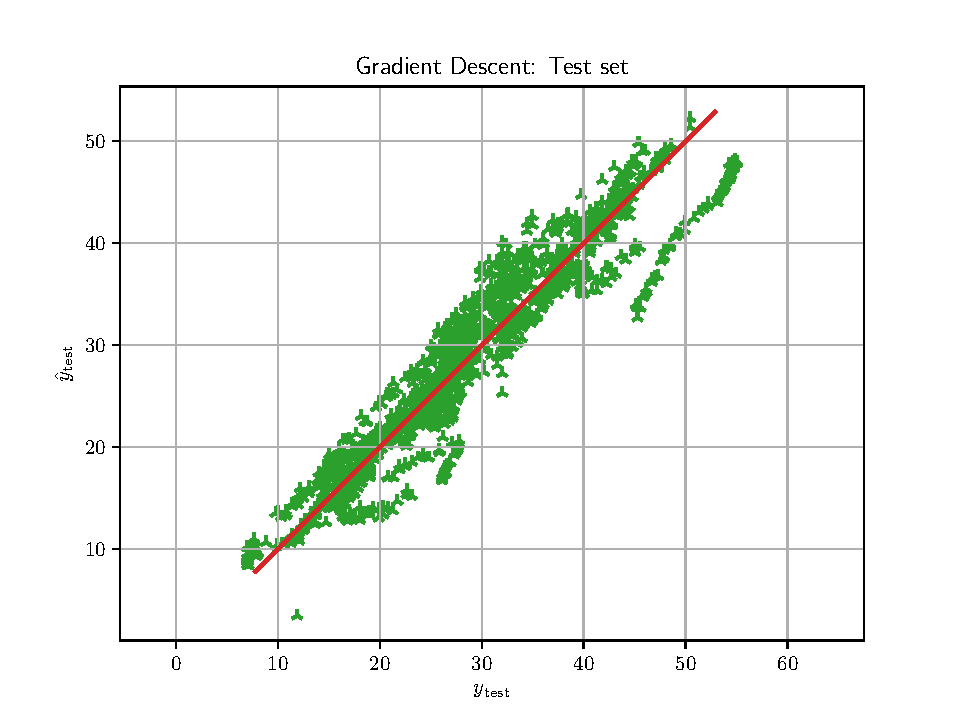
\includegraphics[width=.5\textwidth]{s_test_Gradient_Descent.pdf}}
\subfloat[][\emph{$\hat { \mathbf { y } } _ { \mathrm { test } } \textit{{\scriptsize -} }  \mathbf {y } _ { \mathrm { test } }$}\label{fig:gradd_d}]
{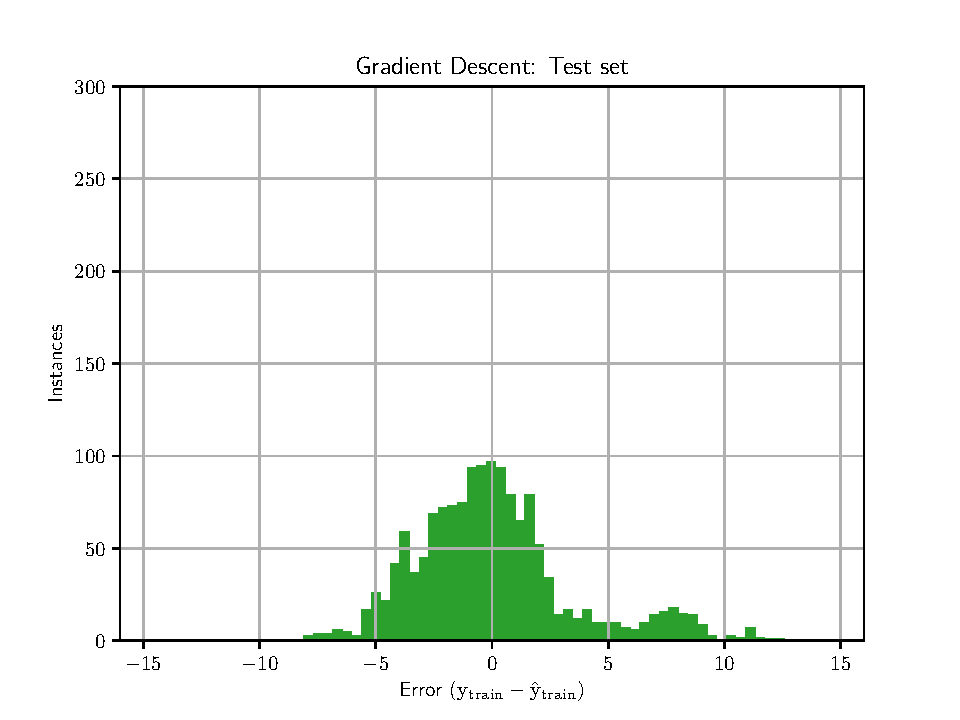
\includegraphics[width=.5\textwidth]{h_test_Gradient_Descent.pdf}}\\
\subfloat[][\emph{Optimum $\textbf{w}$ for every feature}\label{fig:gradd_e}]
{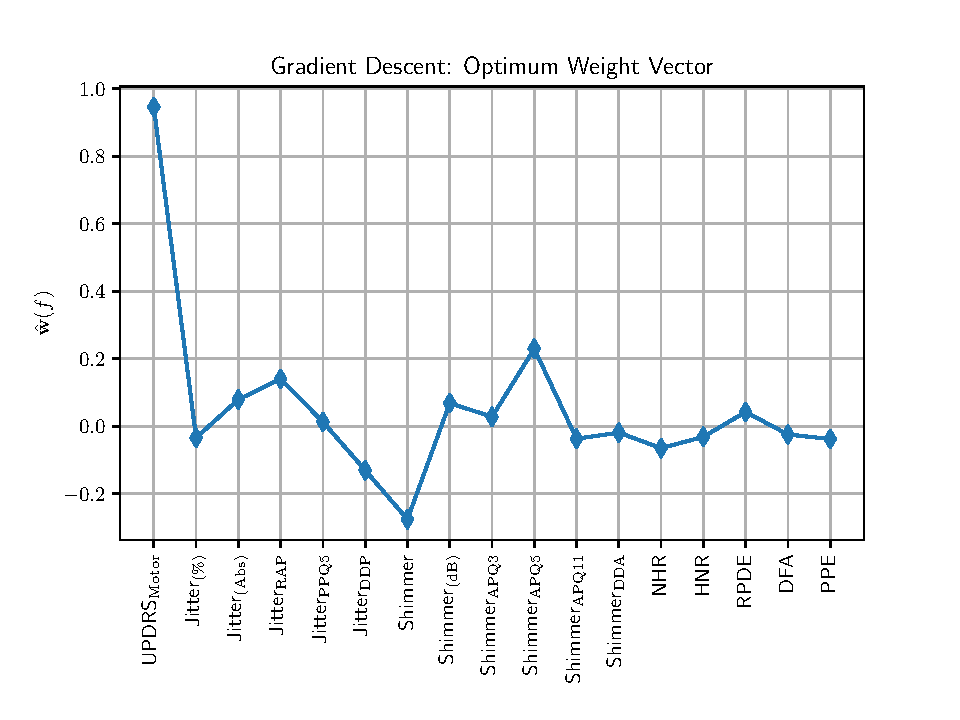
\includegraphics[width=.5\textwidth]{w_Gradient_Descent.pdf}}
\subfloat[][\emph{Mean Square Error}\label{fig:gradd_f}]
{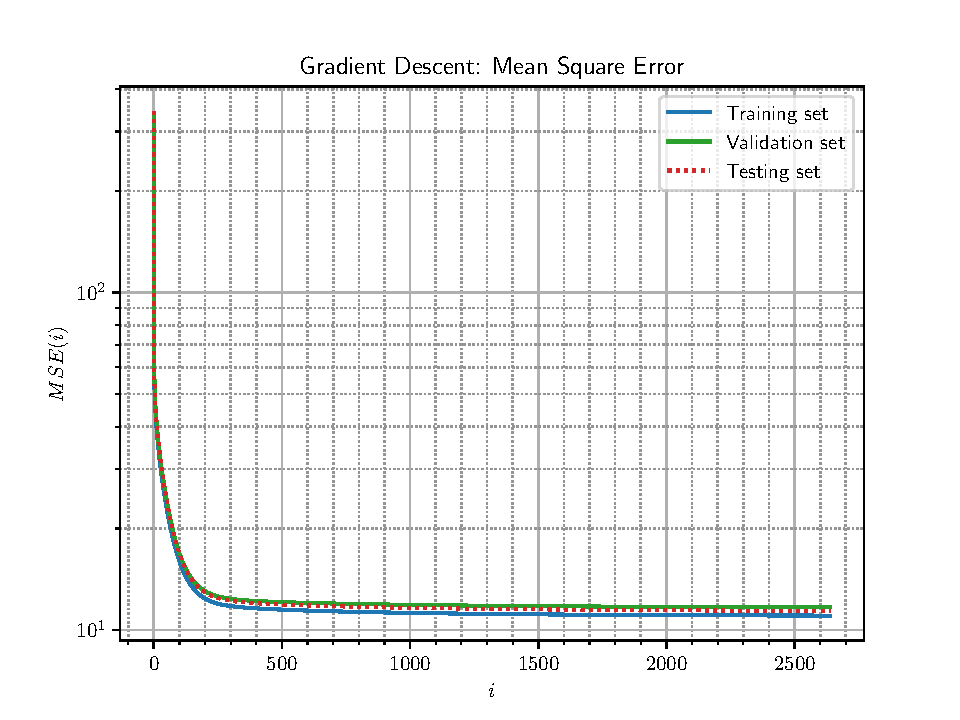
\includegraphics[width=.5\textwidth]{err_Gradient_Descent.pdf}}
\label{fig:gradd}
\caption{Gradient Descent}
\end{figure}




\pagebreak


\section{Steepest Descent}
\begin{wrapfigure}{l}{0.4\textwidth}
  \vspace{-10pt}
  \begin{center}
    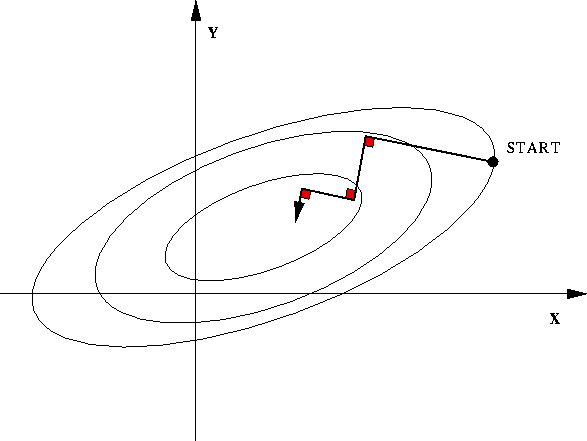
\includegraphics[width=0.4\textwidth]{std.png}
    \caption{Steepest Descent}
    \label{fig:std}
  \end{center}
\end{wrapfigure}
An other algorithm used to find the minimum of a function is the Steepest Descent. The main task with it, is choosing the best learning coefficient $\gamma$. This turns out to be quite tricky. If we use a constant learning coefficient, but make it too small, convergence will be very slow, but if we make it too large, the method can fail to converge at all.
Our goal is always to find the optimum vector \textbf{w} and with this iterative method, we will improve step by step our $\gamma$ by evaluating, for each $\mathbf{x_i}$ the $\nabla f ( \mathbf { x_i } ) $ and the Hessian Matrix in that point: $\mathbf { H } \left( \mathbf { x } _ { i } \right) = 4 \mathbf { X } ^ { T } \mathbf { X }$.

\begin{flushright}
\begin{equation}
\gamma _ { i } = \frac { \left\| \nabla f \left( \mathbf { x } _ { i } \right) \right\| ^ { 2 } } { \nabla f \left( \mathbf { x } _ { i } \right) ^ { T } \mathbf { H } \left( \mathbf { x } _ { i } \right) \nabla f \left( \mathbf { x } _ { i } \right) }
\end{equation}\\


\begin{equation}
\mathbf { x } _ { i + 1 } = \mathbf { x } _ { i } - \frac { \left\| \nabla f \left( \mathbf { x } _ { i } \right) \right\| ^ { 2 } } { \nabla f \left( \mathbf { x } _ { i } \right) ^ { T } \mathbf { H } \left( \mathbf { x } _ { i } \right) \nabla f \left( \mathbf { x } _ { i } \right) } \nabla f \left( \mathbf { x } _ { i } \right)
\end{equation}
\end{flushright}


\subsection{Results}
As in the previous algorithms, in the figures[\textbf{\ref{fig:stepd_a}}] and [\textbf{\ref{fig:stepd_c}}]we see how well the algorithm performs and the enhancement of it is also proven in the figures [\textbf{\ref{fig:stepd_c}}] and [\textbf{\ref{fig:stepd_d}}] where the mean of the error is around $0$.More than in figure [\textbf{\ref{fig:gradd_e}}] we see how crucial is the feature of \texttt{UPDRS}\textsubscript{\textbf{motor}} among the other features which has the highest  in defying, among the other features, the correlation with the \texttt{UPDRS}\textsubscript{\textbf{total}}. The Mean Square Error here performs better than in [\textbf{\ref{fig:gradd_f}}] because the number of iterations required to have a constant trend is only around 50.
\pagebreak

\begin{center}
\subsubsection{Results with the "Steepest Descent" Algorithm}
\end{center}
\begin{figure}[H]
\centering
\begin{center}
\subfloat[][\emph{$\hat { \mathbf { y } } _ { \mathrm { train } } \textit{{\scriptsize VS} }  \mathbf {y } _ { \mathrm { train } }$}\label{fig:stepd_a}]
{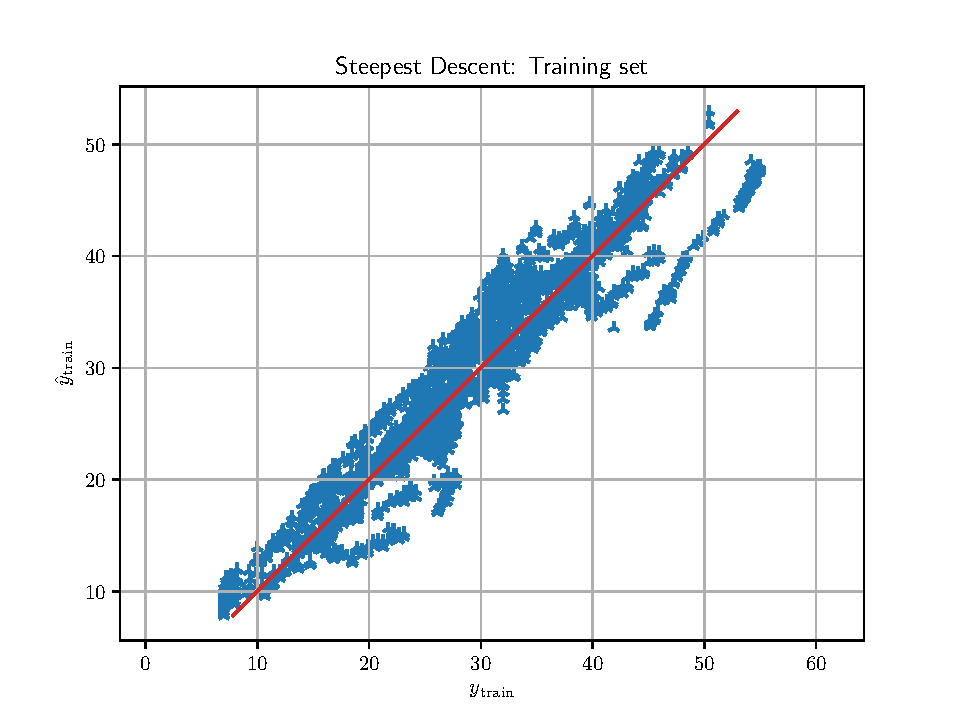
\includegraphics[width=.5\textwidth]{s_train_Steepest_Descent.pdf}}
\subfloat[][\emph{$\hat { \mathbf { y } } _ { \mathrm { train } } \textit{{\scriptsize -} }  \mathbf {y } _ { \mathrm { train } }$}\label{fig:stepd_b}]
{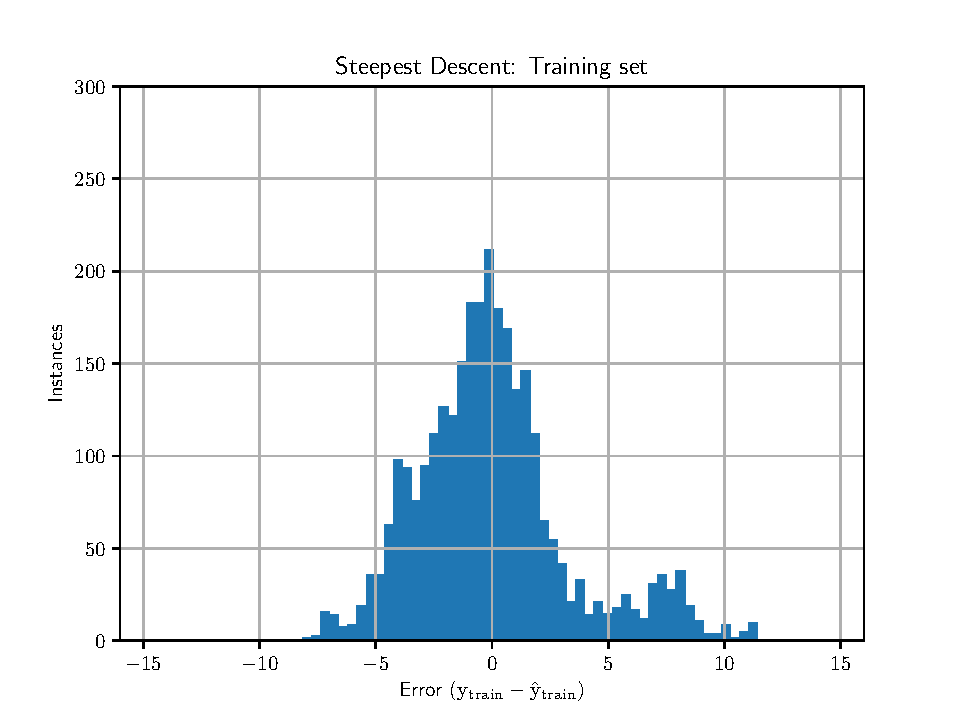
\includegraphics[width=.5\textwidth]{h_train_Steepest_Descent.pdf}}\\
\subfloat[][\emph{$\hat { \mathbf { y } } _ { \mathrm { test } } \textit{{\scriptsize VS} }  \mathbf {y } _ { \mathrm { test } }$}\label{fig:stepd_c}]
{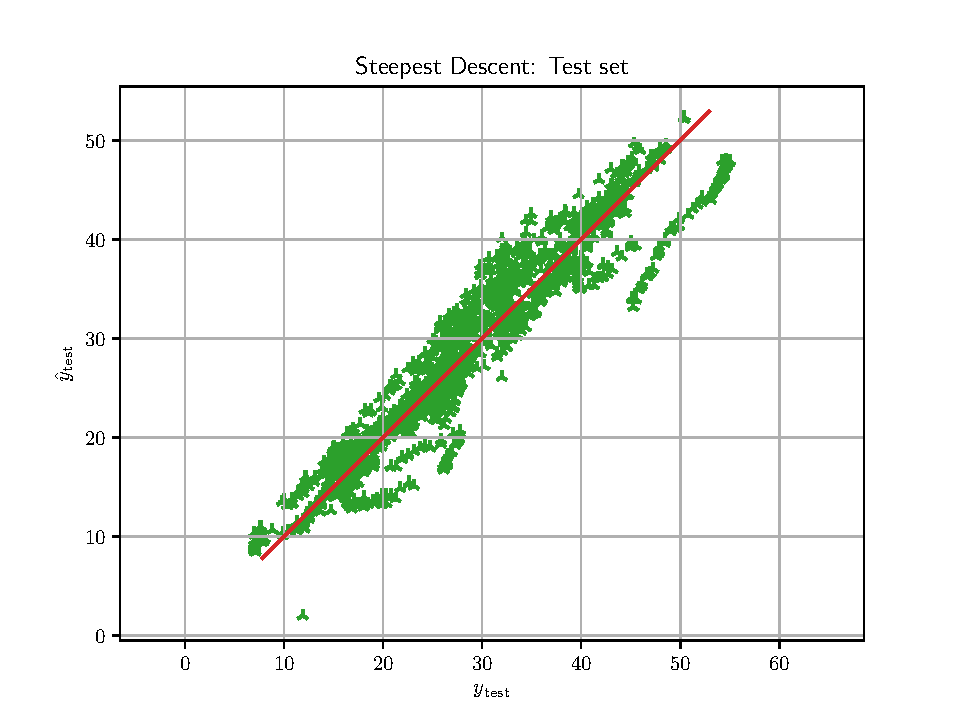
\includegraphics[width=.5\textwidth]{s_test_Steepest_Descent.pdf}}
\subfloat[][\emph{$\hat { \mathbf { y } } _ { \mathrm { test } } \textit{{\scriptsize -} }  \mathbf {y } _ { \mathrm { test } }$}\label{fig:stepd_d}]
{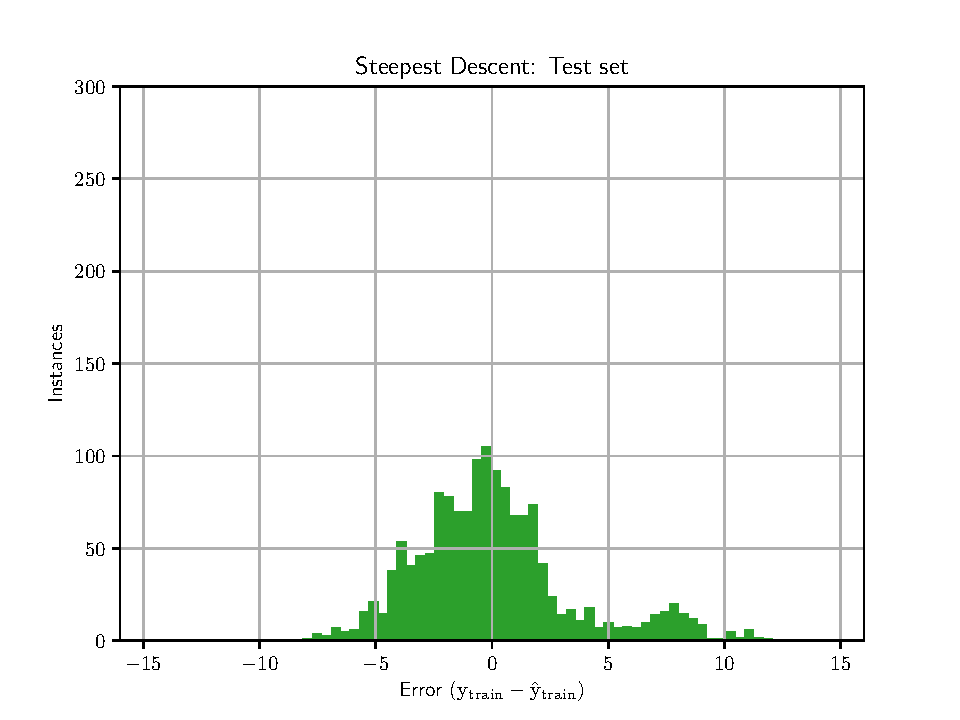
\includegraphics[width=.5\textwidth]{h_test_Steepest_Descent.pdf}}\\
\subfloat[][\emph{Optimum $\textbf{w}$ for every feature}\label{fig:stepd_e}]
{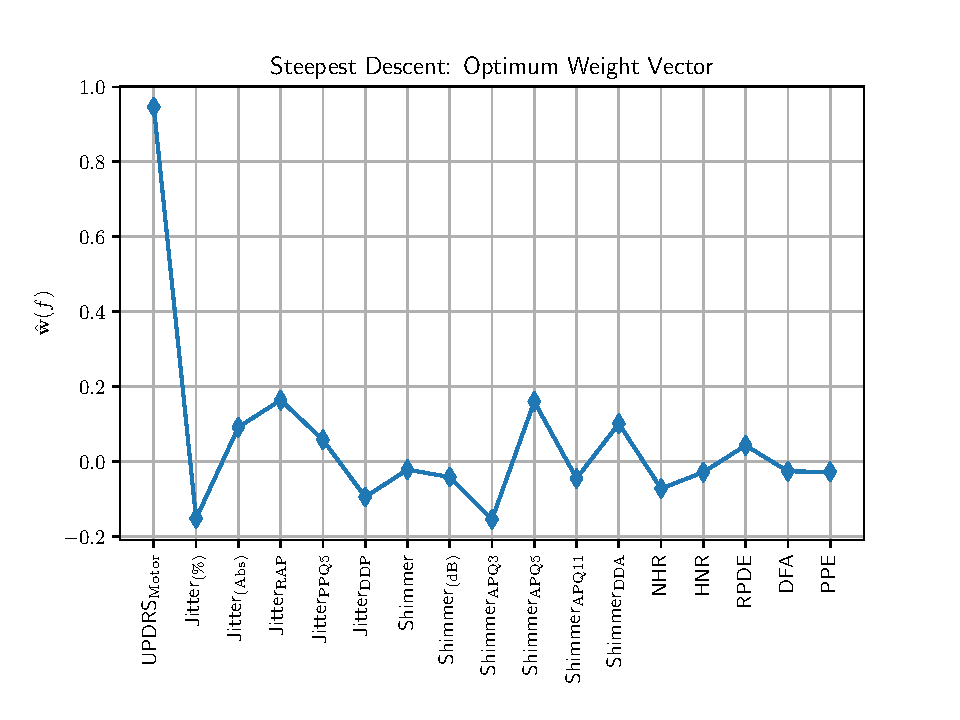
\includegraphics[width=.5\textwidth]{w_Steepest_Descent.pdf}}
\subfloat[][\emph{Mean Square Error}\label{fig:stepd_f}]
{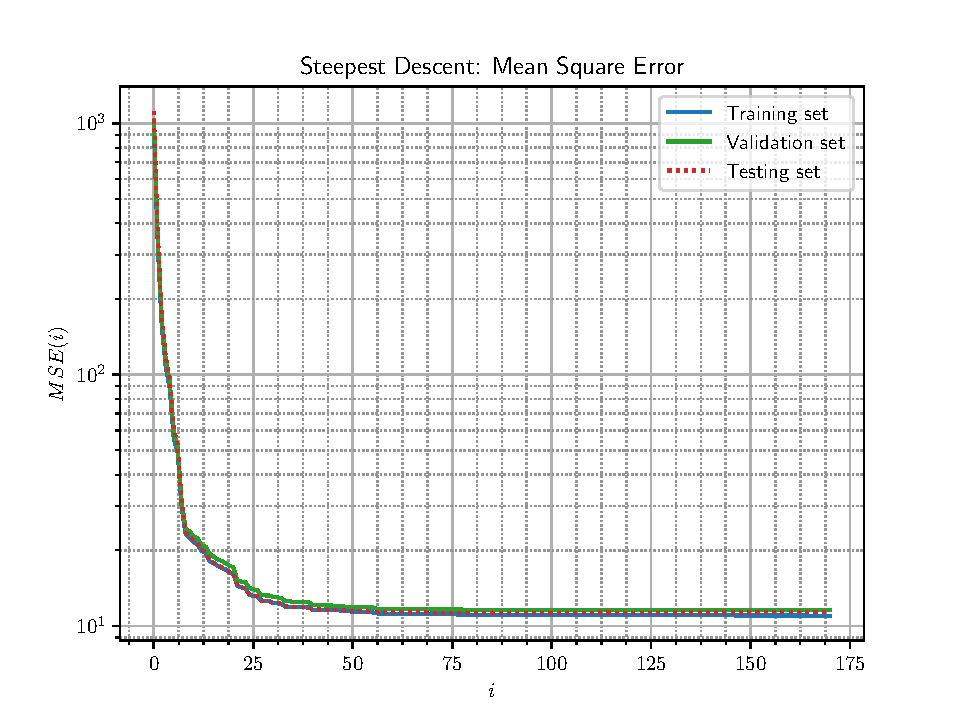
\includegraphics[width=.5\textwidth]{err_Steepest_Descent.pdf}}
\label{fig:stepd}
\caption{Steepest Descent}
\end{center}
\end{figure}

\pagebreak


\section{Stochastic Gradient Descent}
\begin{wrapfigure}{r}{0.3\textwidth}
  \vspace{-35pt}
  \begin{center}
    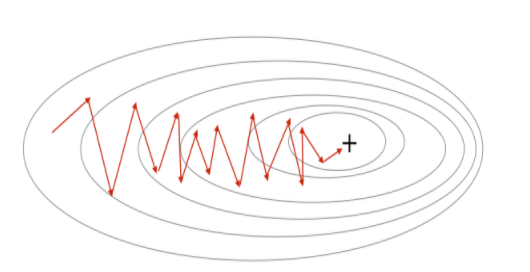
\includegraphics[width=0.25\textwidth]{stch.png}
    \caption{Stochastic Descent}
    \label{fig:stch}
  \end{center}
\end{wrapfigure}
This algorithm it's very similar to the Gradient Descent (\ref{gr}) but the initial approach is totally different. The iterations to find the minimum of the function, start with a stochastically generated $\textbf{w}$.
Our function is defined as in (\ref{2.7}), while the gradient as in (\ref{2.8})
\\\\
\begin{equation}\label{2.7}
f ( \mathbf { w } ) = \| \mathbf { X } \mathbf { w } - \mathbf { y } \| ^ { 2 } = \sum _ { n = 0 } ^ { N }  [ [ \mathbf { x } ( n ) ] ^ { T } \mathbf { w } - y ( n ) ] ^ { 2 } = \sum _ { n = 1 } ^ { N } f _ { n } ( \mathbf { w } )
\end{equation}

\begin{equation}\label{2.8}
\nabla f ( \mathbf { w } ) = \sum _ { n = 0 } ^ { N } \nabla f _ { n } ( \mathbf { w } ) = \sum _ { n = 0 } ^ { N } [ [ \mathbf { x } ( n ) ] ^ { T } \mathbf { w } - y ( n ) ] \mathbf { x } ( n )
\end{equation}\\

Now, as we did in (\ref{2.4}), we iterate until our stopping condition is met:

\begin{equation}\label{2.9}
\mathbf { w } _ { i + 1 } = \mathbf { w } _ { i } - \gamma \nabla f _ { i } ( \mathbf { w } _ { i } )
\end{equation}


\subsection{Results}
Like in sections before, the figures [\textbf{\ref{fig:stog_a}}], [\textbf{\ref{fig:stog_c}}], [\textbf{\ref{fig:stog_b}}]and [\textbf{\ref{fig:stog_d}}] are representative of the good results given by the algorithm; And also here is crucial the amount of importance that the feature \texttt{UPDRS}\textsubscript{\textbf{motor}}, in figure [\textbf{\ref{fig:stog_e}}], has in the regression analysis. The particularity of this algorithm is, as we said in the initial description of it, that it updates the vector w using an estimate of the gradient based on the single rows of the matrix. The evaluation will surely be faster but not so accurate and this is because it takes so much time to reach convergence. For each iteration shown in figure [\textbf{\ref{fig:stog_f}}] the algorithm evaluated the gradient 2938 times that is the number of rows of the $\textbf{X}_{train}$ matrix.
\pagebreak

\begin{center}
\subsubsection{Results with the "Stochastic Gradient Descent" Algorithm}
\end{center}
\begin{figure}[H]
\centering
\begin{center}
\subfloat[][\emph{$\hat { \mathbf { y } } _ { \mathrm { train } } \textit{{\scriptsize VS} }  \mathbf {y } _ { \mathrm { train } }$}\label{fig:stog_a}]
{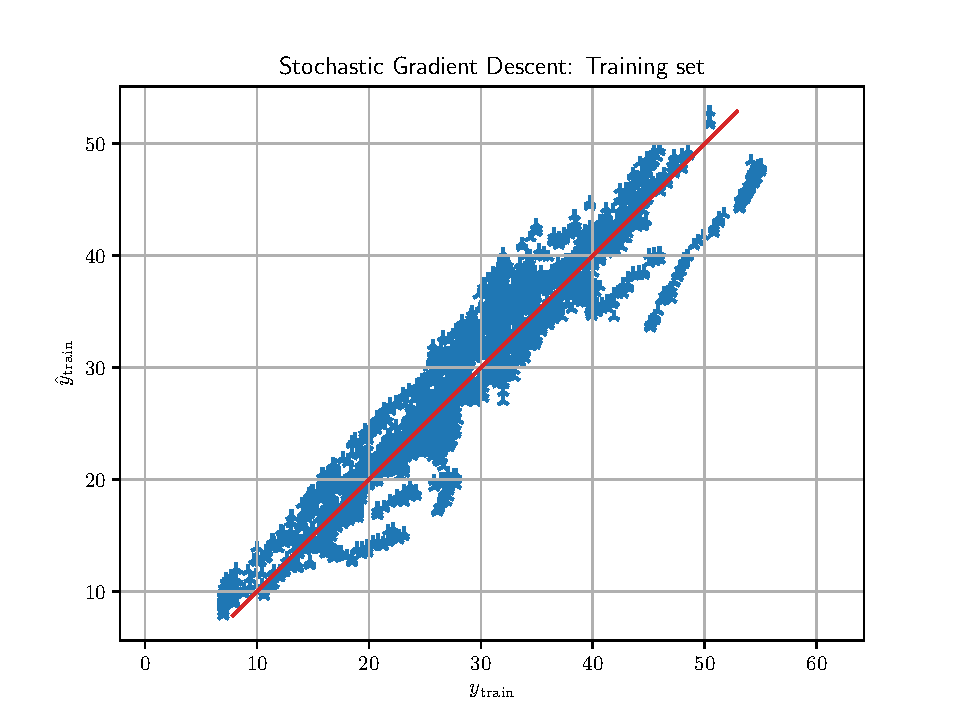
\includegraphics[width=.5\textwidth]{s_train_Stochastic_Gradient_Descent.pdf}}
\subfloat[][\emph{$\hat { \mathbf { y } } _ { \mathrm { train } } \textit{{\scriptsize -} }  \mathbf {y } _ { \mathrm { train } }$}\label{fig:stog_b}]
{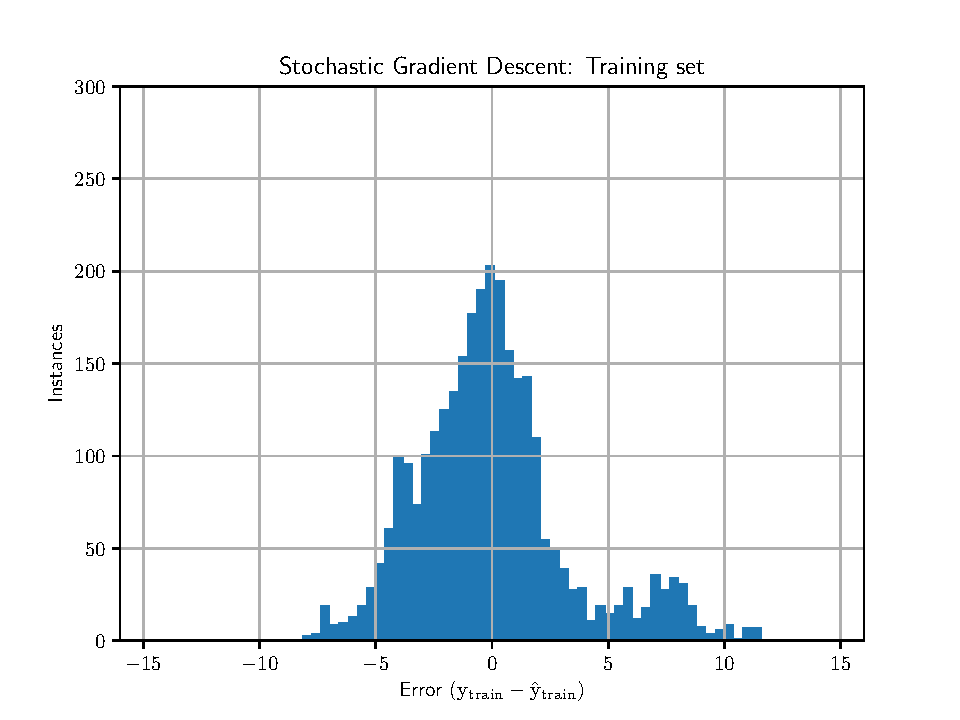
\includegraphics[width=.5\textwidth]{h_train_Stochastic_Gradient_Descent.pdf}}\\
\subfloat[][\emph{$\hat { \mathbf { y } } _ { \mathrm { test } } \textit{{\scriptsize VS} }  \mathbf {y } _ { \mathrm { test } }$}\label{fig:stog_c}]
{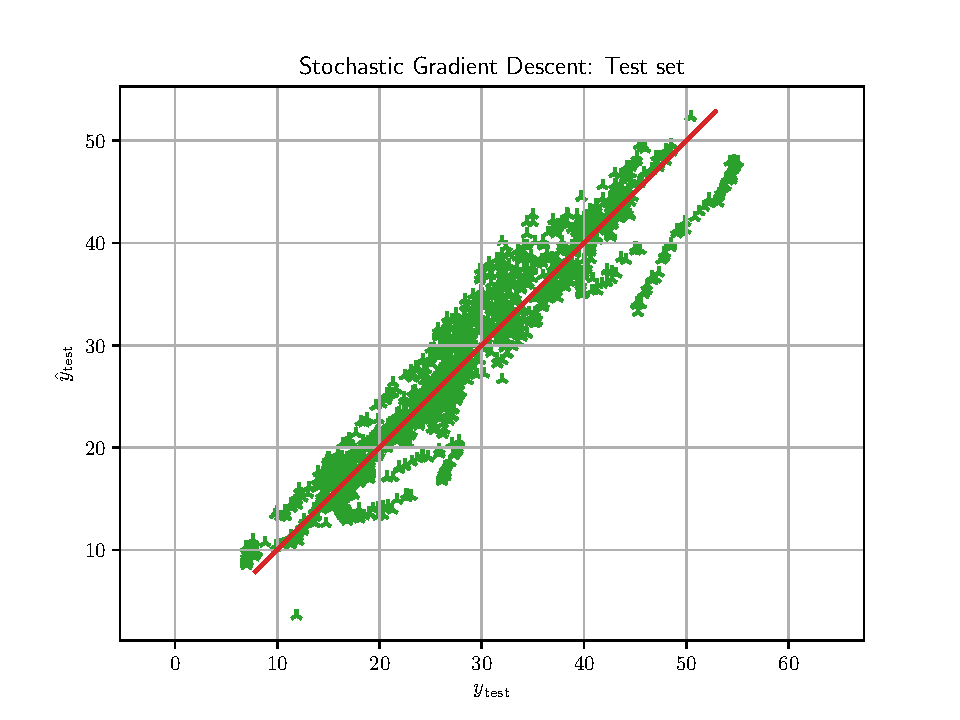
\includegraphics[width=.5\textwidth]{s_test_Stochastic_Gradient_Descent.pdf}}
\subfloat[][\emph{$\hat { \mathbf { y } } _ { \mathrm { test } } \textit{{\scriptsize -} }  \mathbf {y } _ { \mathrm { test } }$}\label{fig:stog_d}]
{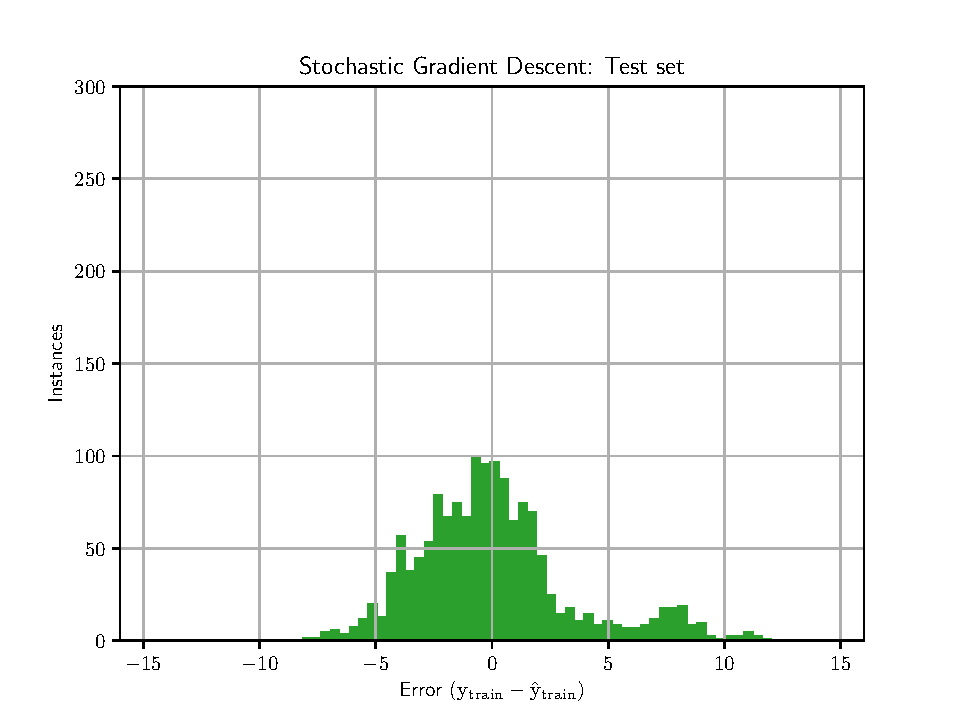
\includegraphics[width=.5\textwidth]{h_test_Stochastic_Gradient_Descent.pdf}}\\
\subfloat[][\emph{Optimum $\textbf{w}$ for every feature}\label{fig:stog_e}]
{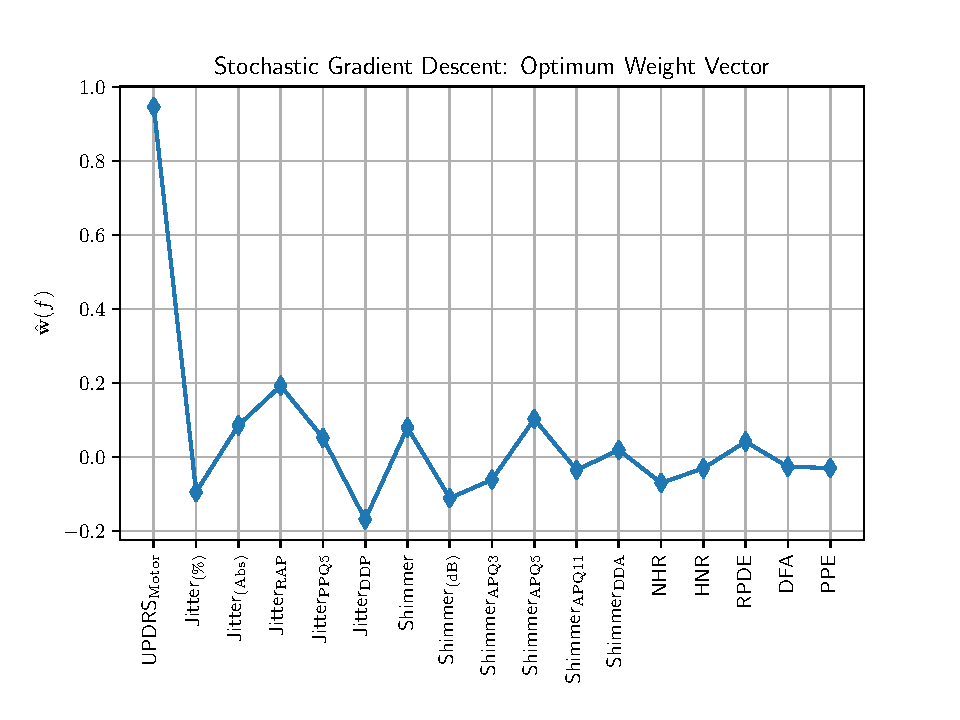
\includegraphics[width=.5\textwidth]{w_Stochastic_Gradient_Descent.pdf}}
\subfloat[][\emph{Mean Square Error}\label{fig:stog_f}]
{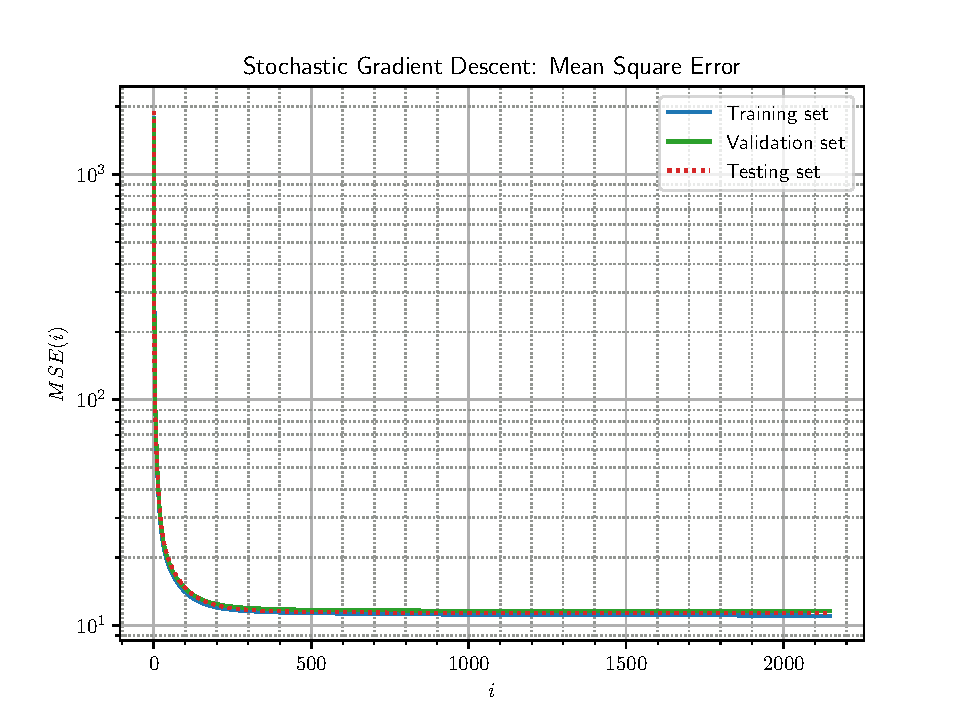
\includegraphics[width=.5\textwidth]{err_Stochastic_Gradient_Descent.pdf}}
\label{fig:stog}
\caption{Stochastic Gradient Descent}
\end{center}
\end{figure}

\pagebreak

\section{Conjugate Gradient Descent}



The conjugate gradient method operates similarly to the gradient descent. The difference is that the directions taken after each iteration are the conjugate of the previous ones. This leads to a very fast convergence since it skips a lot of steps that the gradient descent would have made \cite{conjjj}.

The problem to solve is \eqref{eq:conjprobl}:
\begin{equation}
\label{eq:conjprobl}
\vec{Q}\vec{w}^*-\vec{b}=0
\end{equation}
A solution can be found with the help of \emph{conjugate vectors} which are vectors orthogonal with respect to a matrix $\vec{Q}$. It means that the vectors $\vec{d}_i$ and $\vec{d}_k$ are Q-orthogonal if $\vec{d}_i^T\vec{Q}\vec{d}_k=0$.


At first we set $\vec{d}_0=-\vec{g}_0=\vec{b}$ and $\vec{w}_0=0$ as the initial solution, where $\vec{g}$ is the direction of the gradient and $\vec{d}$ is the actual direction taken by the algorithm.
The next directions are computed as $\vec{d}_{k+1}=-\vec{g}_{k+1}+\beta_{k}\vec{d}_k$ where $\beta$ is a coefficient that depends on the other parameters.

The algorithm converges in $N_{f}$ steps where $N_{f}$ is the dimension of the problem.


\subsection{Results}
The good results of this algorithm are not only explained by the plots [\textbf{\ref{fig:conj_a}}] and [\textbf{\ref{fig:conj_c}}] and by the histograms of figure[\textbf{\ref{fig:conj_b}}] and [\textbf{\ref{fig:conj_d}}] but especially by the Mean Square Error graph [\textbf{\ref{fig:conj_f}}]. The Conjugate Gradient Method, with just few iterations, is able to reach a constant train (in our case it has stopped after 17 iterations) and the amount of overfitting is visible only in the first few iterations.

\pagebreak

\begin{center}
\subsubsection{Results with the "Conjugate Gradient Descent" Algorithm}
\end{center}
\begin{figure}[H]
\centering
\begin{center}
\subfloat[][\emph{$\hat { \mathbf { y } } _ { \mathrm { train } } \textit{{\scriptsize VS} }  \mathbf {y } _ { \mathrm { train } }$}\label{fig:conj_a}]
{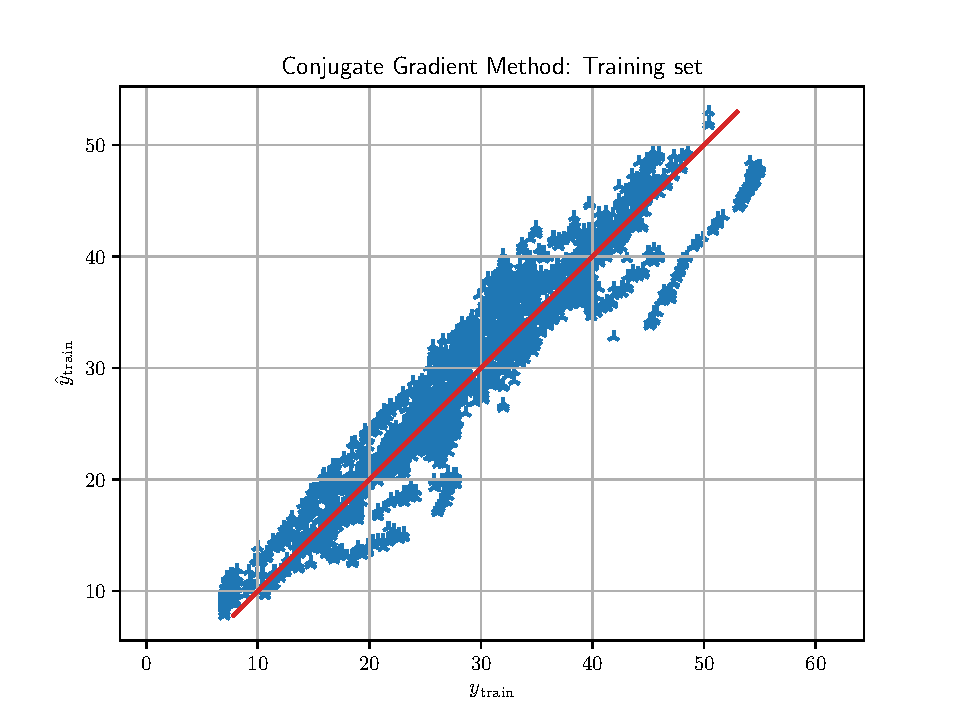
\includegraphics[width=.5\textwidth]{s_train_Conjugate_Gradient_Method.pdf}}
\subfloat[][\emph{$\hat { \mathbf { y } } _ { \mathrm { train } } \textit{{\scriptsize -} }  \mathbf {y } _ { \mathrm { train } }$}\label{fig:conj_b}]
{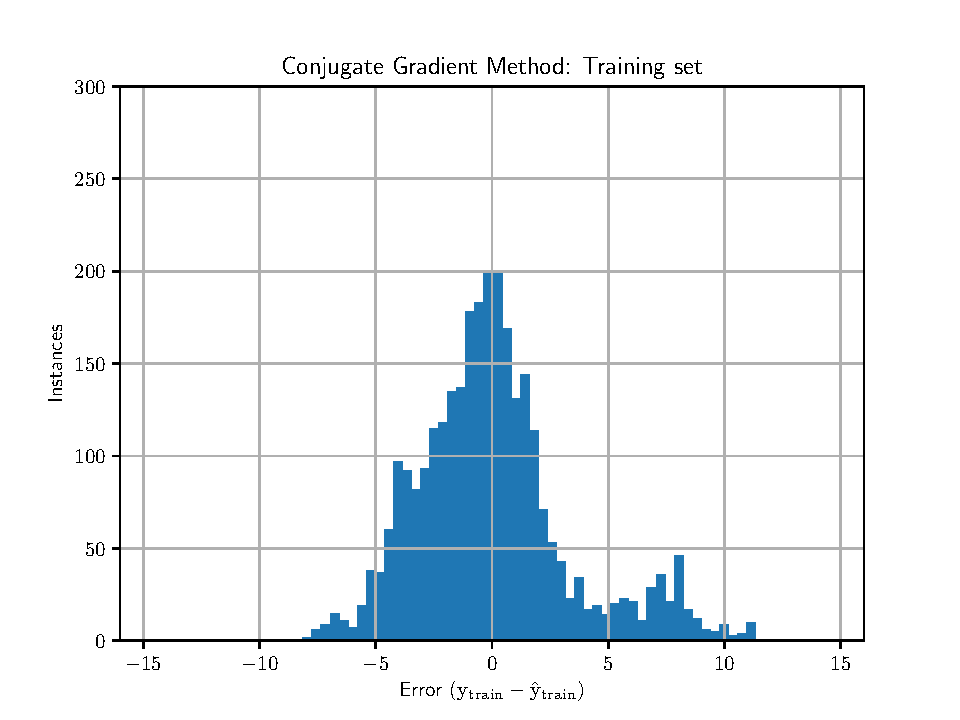
\includegraphics[width=.5\textwidth]{h_train_Conjugate_Gradient_Method.pdf}}\\
\subfloat[][\emph{$\hat { \mathbf { y } } _ { \mathrm { test } } \textit{{\scriptsize VS} }  \mathbf {y } _ { \mathrm { test } }$}\label{fig:conj_c}]
{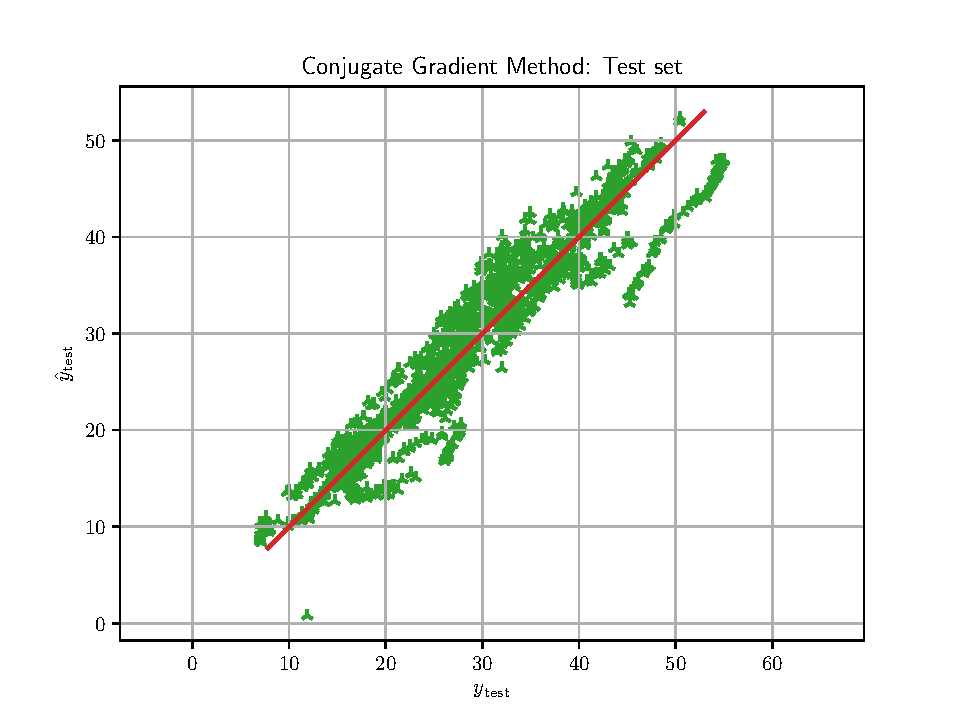
\includegraphics[width=.5\textwidth]{s_test_Conjugate_Gradient_Method.pdf}}
\subfloat[][\emph{$\hat { \mathbf { y } } _ { \mathrm { test } } \textit{{\scriptsize -} }  \mathbf {y } _ { \mathrm { test } }$}\label{fig:conj_d}]
{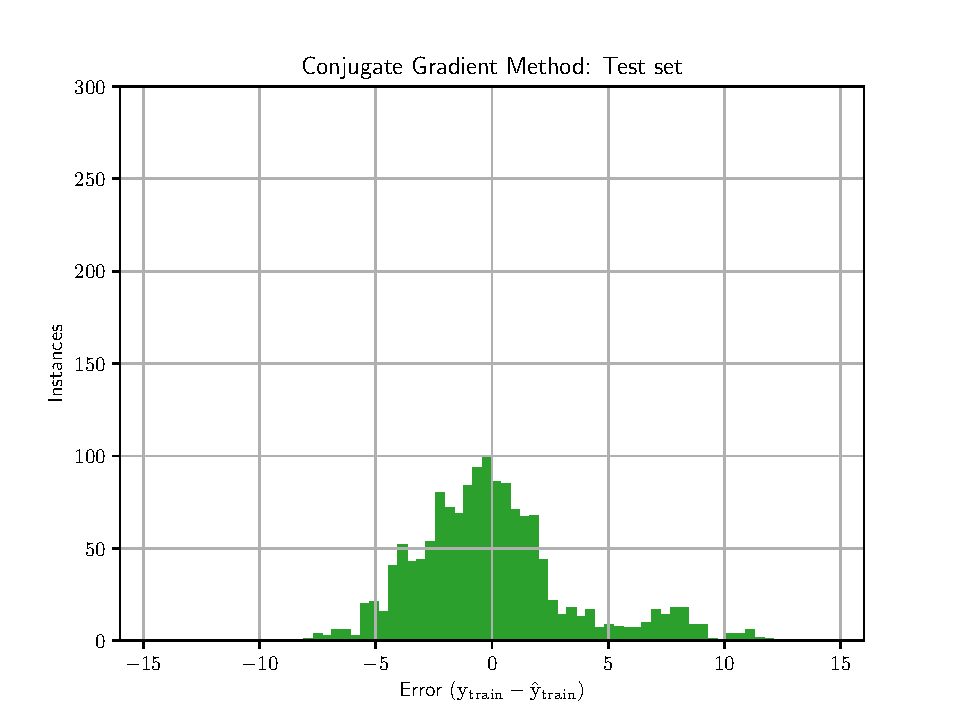
\includegraphics[width=.5\textwidth]{h_test_Conjugate_Gradient_Method.pdf}}\\
\subfloat[][\emph{Optimum $\textbf{w}$ for every feature}\label{fig:conj_e}]
{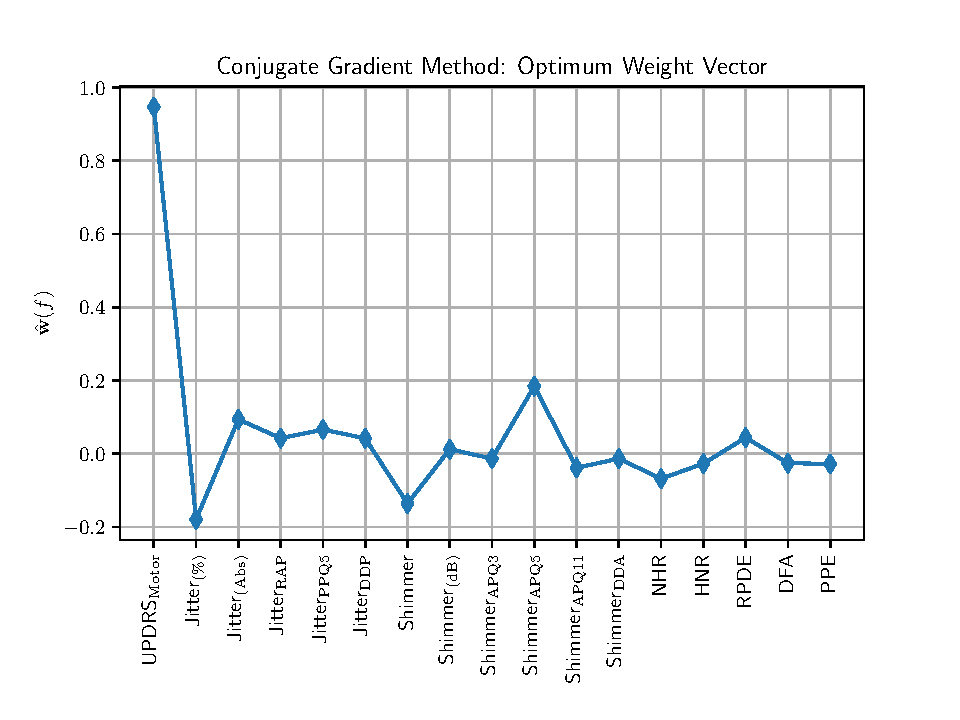
\includegraphics[width=.5\textwidth]{w_Conjugate_Gradient_Method.pdf}}
\subfloat[][\emph{Mean Square Error}\label{fig:conj_f}]
{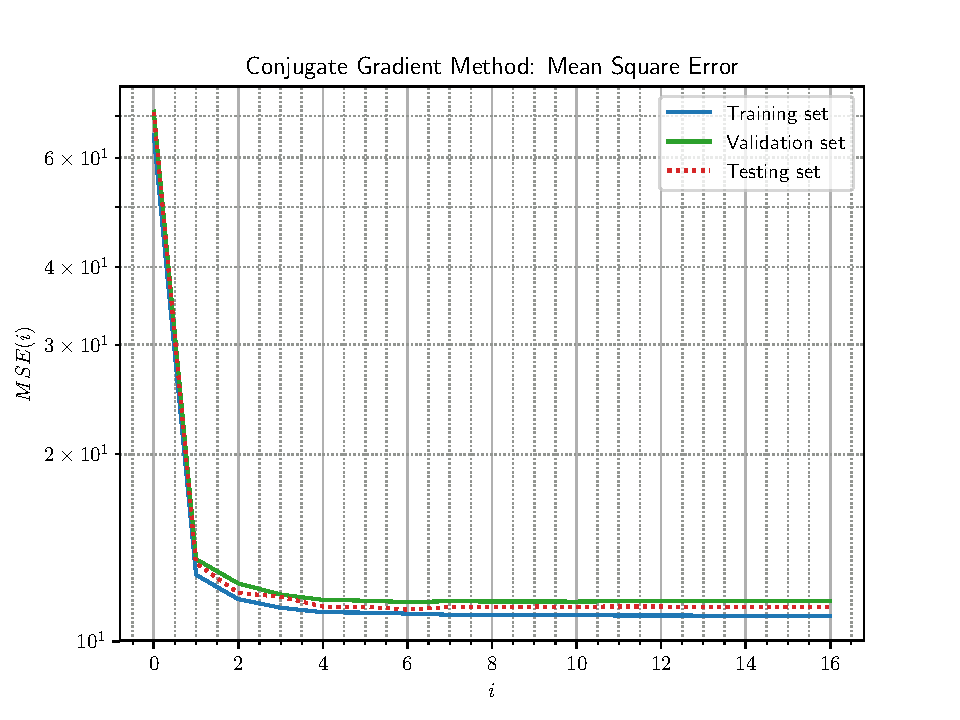
\includegraphics[width=.5\textwidth]{err_Conjugate_Gradient_Method.pdf}}
\label{fig:conj}
\caption{Conjugate Gradient Descent}
\end{center}
\end{figure}

\pagebreak


\section{Ridge Regression \cite{MV}}
If $ \mathbf { y } = \mathbf { X } \mathbf { w } + \boldsymbol { \nu } $ has some large values of noise/error, it is possible that vector $\mathbf { \hat { w } }$ takes very large values and overfitting occurs. Then, it might be convenient to solve the new problem:

\begin{equation}
\operatorname { min } _ { \mathbf { w } } \| \mathbf { y } - \mathbf { X } \mathbf { w } \| ^ { 2 } + \lambda \| \mathbf { w } \| ^ { 2 } = \operatorname { min } _ { \mathbf { w } } f ( \mathbf { w } )
\end{equation}\\
where $\mu$ has to be set conveniently (trial and error). The solution of this problem can then be obtained using the pseudoinverse, in fact

\begin{equation}
\nabla f ( \mathbf { w } ) = 2 \mathbf { X } ^ { \top } \mathbf { X } \mathbf { w } - 2 \mathbf { X } ^ { \top } \mathbf { y } + 2 \lambda \mathbf { w } = 0
\end{equation}


\begin{equation}
\hat { \mathbf { w } } = \left( \mathbf { X } ^ { \top } \mathbf { X } + \lambda \mathbf { I } \right) ^ { - 1 } \mathbf { X } ^ { \top } \mathbf { y }
\end{equation}


\subsection{Results}
With this algorithm we tried to find the best result by choosing the best $\lambda$ between $[0,80]$. The result for us was $\lambda =6.835085$ , since in our case it is the value that minimizes the mean squared error on the validation set, as we can see in figure [\textbf{\ref{fig:rid_f}}]. The rest of the figures, similarly as before, are significant of the good work of the algorithm in doing regression analysis.


\pagebreak

\begin{center}
\subsubsection{Results with the "Ridge Regression" Algorithm}
\end{center}
\begin{figure}[H]
\centering
\begin{center}
\subfloat[][\emph{$\hat { \mathbf { y } } _ { \mathrm { train } } \textit{{\scriptsize VS} }  \mathbf {y } _ { \mathrm { train } }$}\label{fig:rid_a}]
{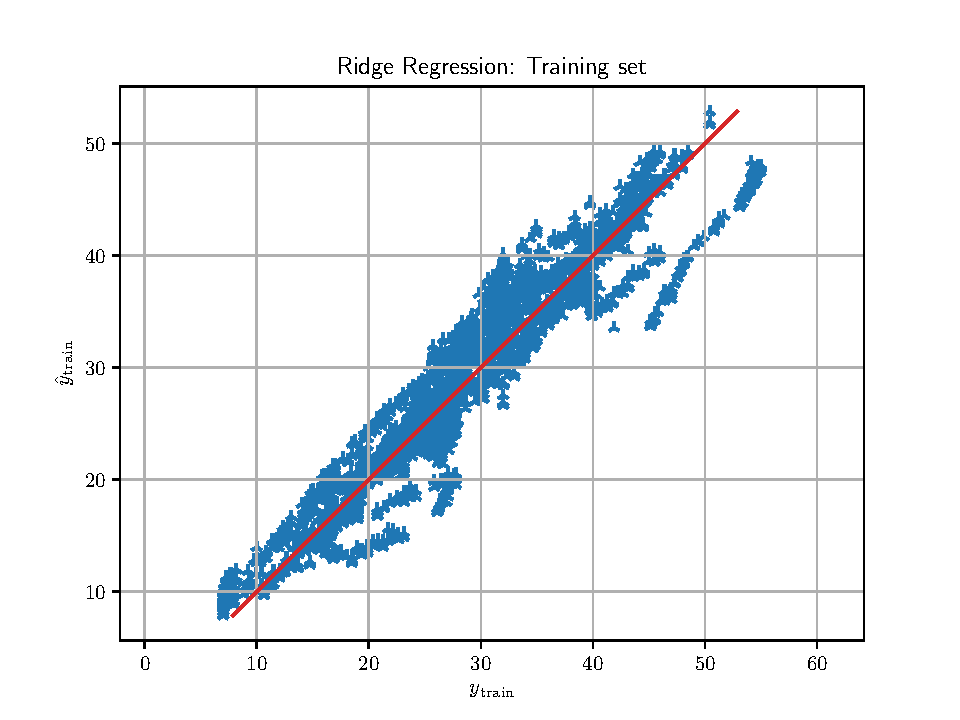
\includegraphics[width=.5\textwidth]{s_train_Ridge_Regression.pdf}}
\subfloat[][\emph{$\hat { \mathbf { y } } _ { \mathrm { train } } \textit{{\scriptsize -} }  \mathbf {y } _ { \mathrm { train } }$}\label{fig:rid_b}]
{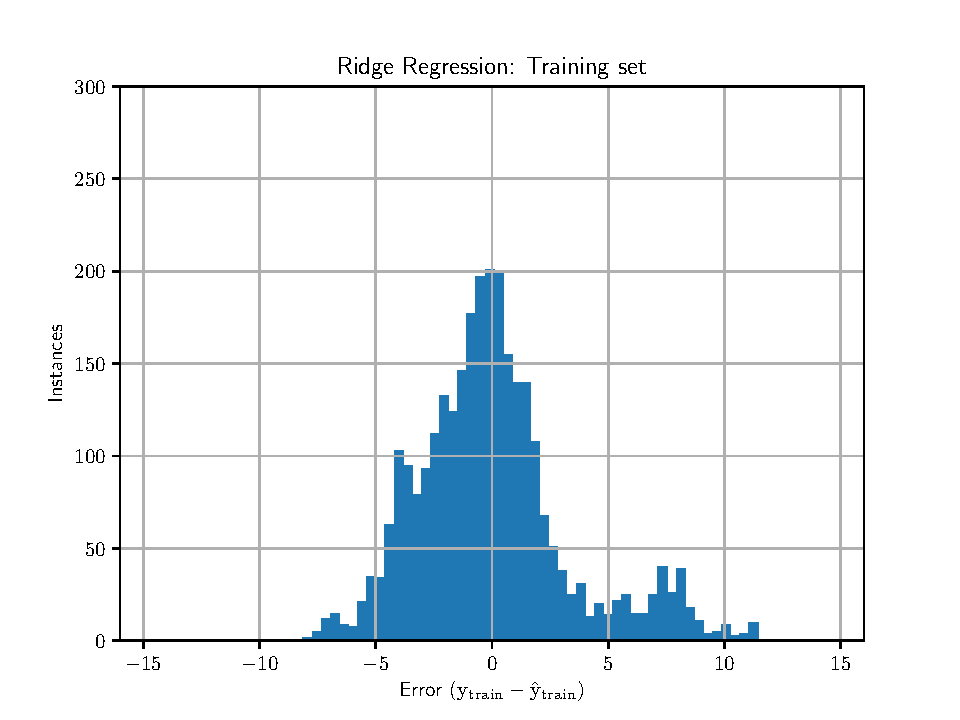
\includegraphics[width=.5\textwidth]{h_train_Ridge_Regression.pdf}}\\
\subfloat[][\emph{$\hat { \mathbf { y } } _ { \mathrm { test } } \textit{{\scriptsize VS} }  \mathbf {y } _ { \mathrm { test } }$}\label{fig:rid_c}]
{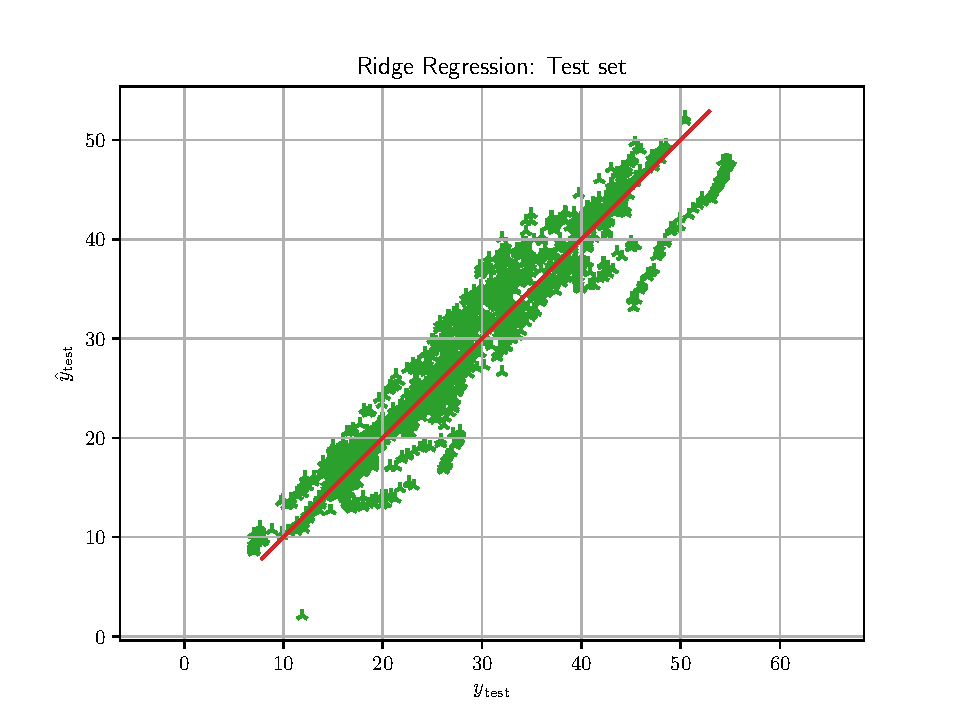
\includegraphics[width=.5\textwidth]{s_test_Ridge_Regression.pdf}}
\subfloat[][\emph{$\hat { \mathbf { y } } _ { \mathrm { test } } \textit{{\scriptsize -} }  \mathbf {y } _ { \mathrm { test } }$}\label{fig:rid_d}]
{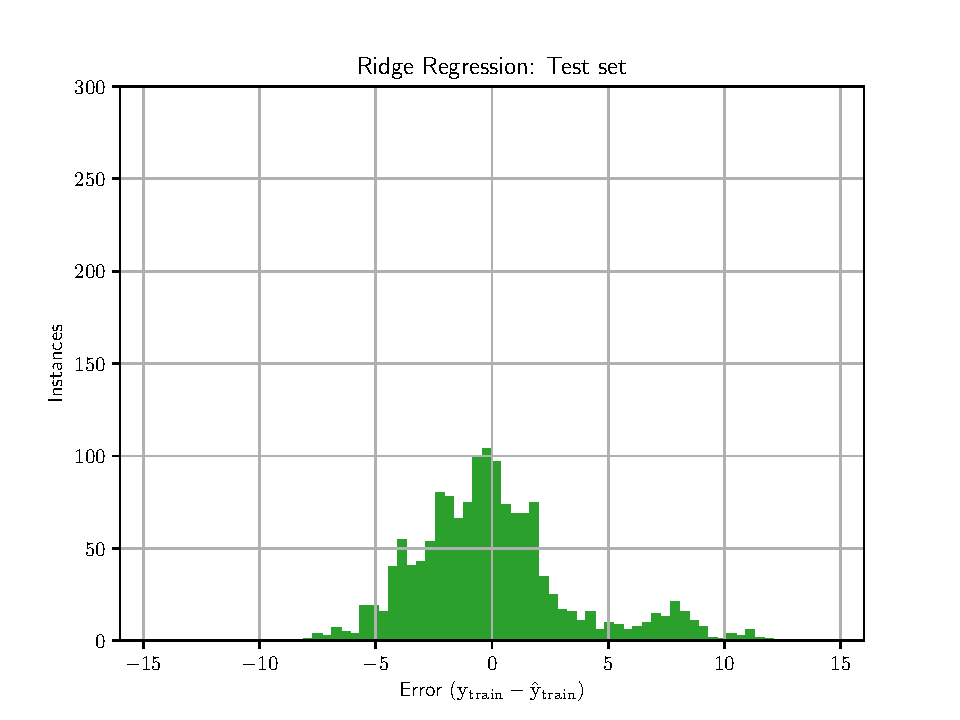
\includegraphics[width=.5\textwidth]{h_test_Ridge_Regression.pdf}}\\
\subfloat[][\emph{Optimum $\textbf{w}$ for every feature}\label{fig:rid_e}]
{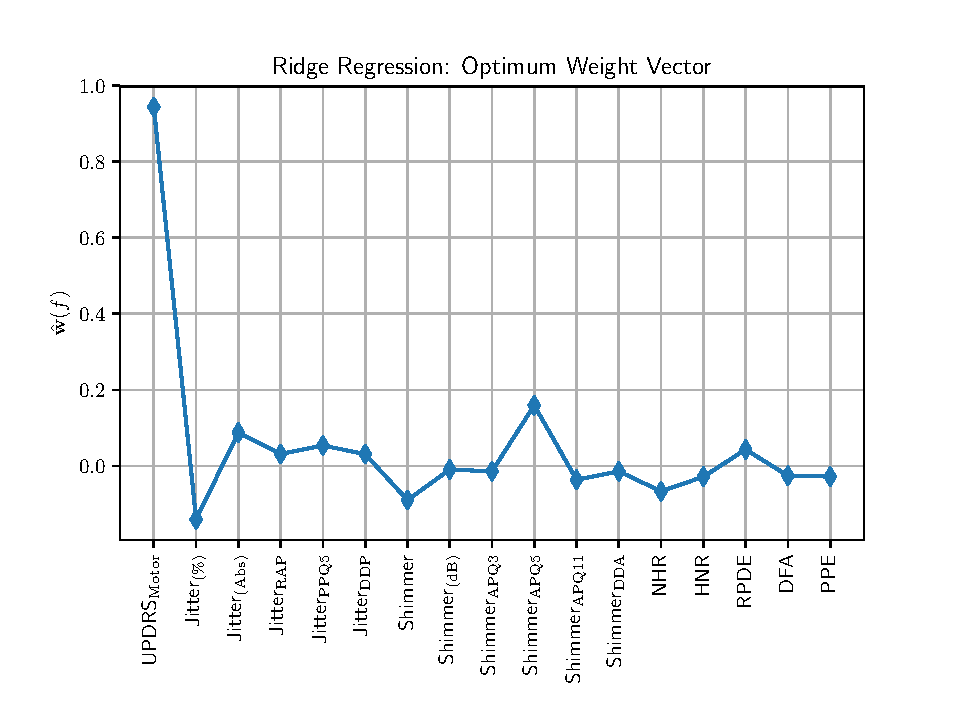
\includegraphics[width=.5\textwidth]{w_Ridge_Regression.pdf}}
\subfloat[][\emph{Mean Square Error}\label{fig:rid_f}]
{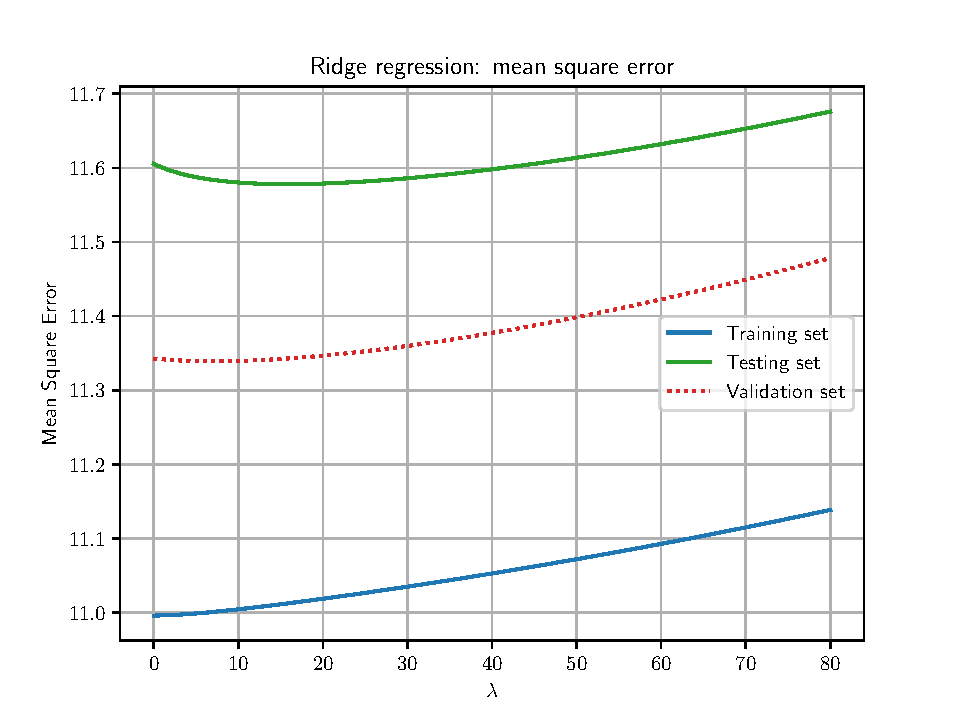
\includegraphics[width=.5\textwidth]{err_Ridge_Regression.pdf}}
\label{fig:rid}
\caption{Ridge Regression}
\end{center}
\end{figure}

\pagebreak

\chapter{ Comparisons beetween the algorithms}

To conclude we saw how, among all the features of the data matrix, \texttt{UPDRS}\textsubscript{\textbf{motor}} was the most significant one for the regression on the \texttt{UPDRS}\textsubscript{\textbf{total}} feature.
Table 3.1 shows the mean squared errors for each algorithm and each dataset. We can see that the MSE for the training set is always the lowest one, due to the fact that the optimum weight vector is evaluated on the training set itself. The mean squared errors on the test and validation sets do not differ too much since they contain the same $\hat{\textbf{w}}$.



\begin{table}[]\label{hello}
\resizebox{\textwidth}{!}{%
\begin{tabular}{|c|c|c|c|c|}
\hline
\textbf{Algorithm} & \textbf{Iterations} & \textbf{Training MSE} & \textbf{Testing MSE} & \textbf{Validation MSE} \\ \hline
Linear Least Square & 1 & 10.9960 & 11.6060 & 11.3431 \\ \hline
Gradient Descent & 2641 & 11.0363 & 11.6739 & 11.3950 \\ \hline
Steepest Descent & 172 & 11.0046 & 11.5785 & 11.3496 \\ \hline
Stochastic Gradient Descent & 6312400 & 11.0413 & 11.5692 & 11.3542 \\ \hline
Conjugate Gradient Descent & 17 & 10.9961 & 11.6053 & 11.3429 \\ \hline
Ridge Regression & 1 & 11.0008 & 11.5840 & 11.3391 \\ \hline
\end{tabular}%
}
\caption{Final results in terms of MSE and Number of Iterations for Training, Testing and Validation Data}
\end{table}



\pagebreak

\pagenumbering{gobble}

\begin{thebibliography}{99}
\bibitem{WikiRegression} \texttt{Regression Analysis}\\\url{https://en.wikipedia.org/wiki/Regression_analysis}
\bibitem{site} \texttt{Machine Learning Data}\\\url{https://archive.ics.uci.edu/ml/datasets/Parkinsons+Telemonitoring}
\bibitem{GD} \texttt{Gradient Descent}\\\url{https://en.wikipedia.org/wiki/Gradient_descent}
\bibitem{MV1} \texttt{ICT for Health Laboratory 1: Regression on Parkinson data}\\\url{https://didattica.polito.it/pls/portal30/sviluppo.scheda_pers_swas.show?m=1834}
\bibitem{MV} \texttt{Linear Regression: Slides of Lecture 3}\\ \url{https://didattica.polito.it/pls/portal30/sviluppo.scheda_pers_swas.show?m=1834}
\bibitem{conjjj} \texttt{On My Phd:\textit{ Conjugate Gradient Method}}\\ \url{http://www.onmyphd.com/?p=conjugate.gradient.method}
\end{thebibliography}


\end{document}
